% NX506 mid-air
\clearpage
\invisiblesection{Figures}

\begin{figure}[t!]
        \centering
        
        \caption[Measurement results {\nexus} (6), mid-air]{{\nexus}, labelled with number 6, measurements in mid-air, equalized}
        \label{fig:res_NX506_pluis}

        \begin{subfigure}[t]{0.5\textwidth}
			    \caption{$\phi=90^\circ$}
			    \label{fig:res_NX506_pluis_90}
                \centering
    			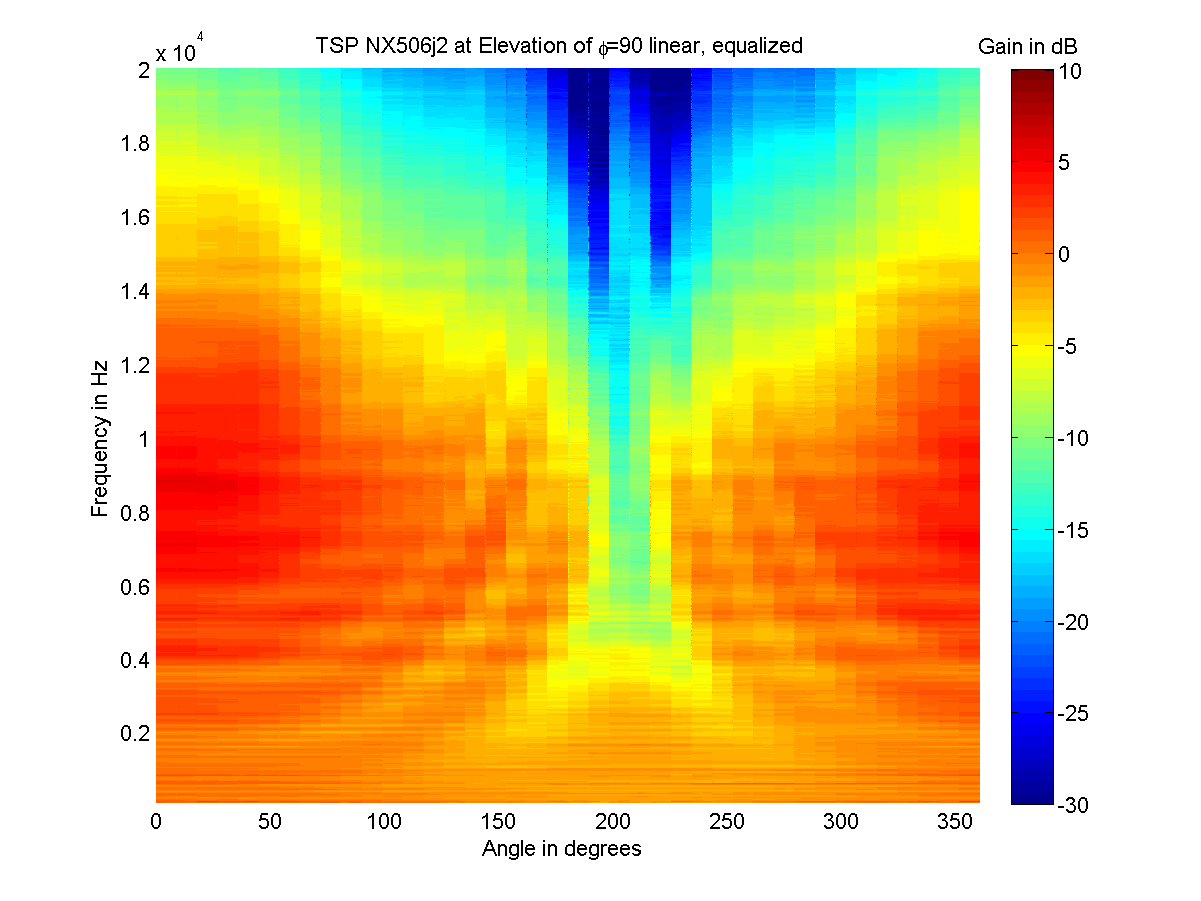
\includegraphics[height=0.28\textheight]{afbeeldingen/plots/results/NX506j2_TSP_090_lin_eq.png}
        \end{subfigure}~
        \begin{subfigure}[t]{0.5\textwidth}
			    \caption{$\phi=42^\circ$}
			    \label{fig:res_NX506_pluis_42}
                \centering
    			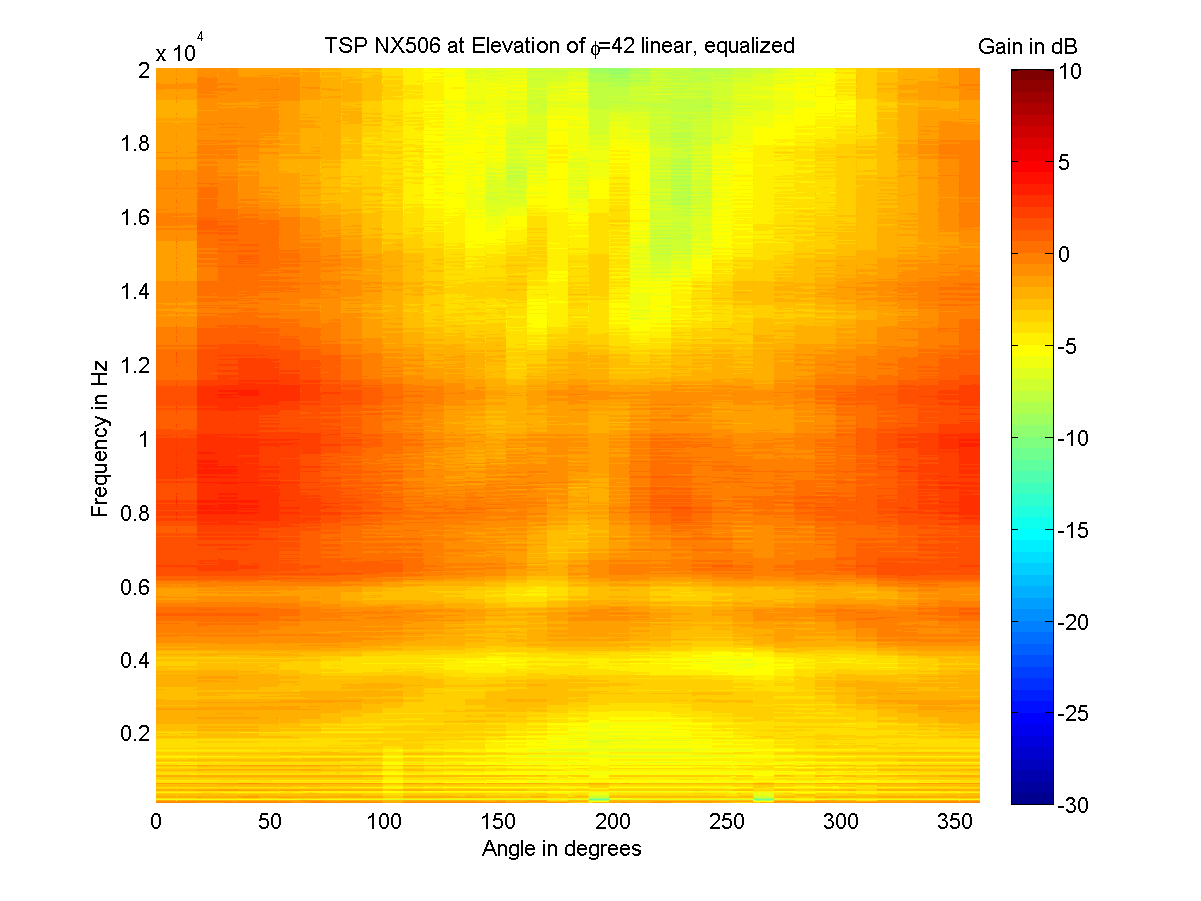
\includegraphics[height=0.28\textheight]{afbeeldingen/plots/results/NX506_TSP_042_lin_eq.png}
        \end{subfigure}
        
        \begin{subfigure}[t]{0.5\textwidth}
			    \caption{$\phi=138^\circ$}
			    \label{fig:res_NX506_pluis_138}
                \centering
    			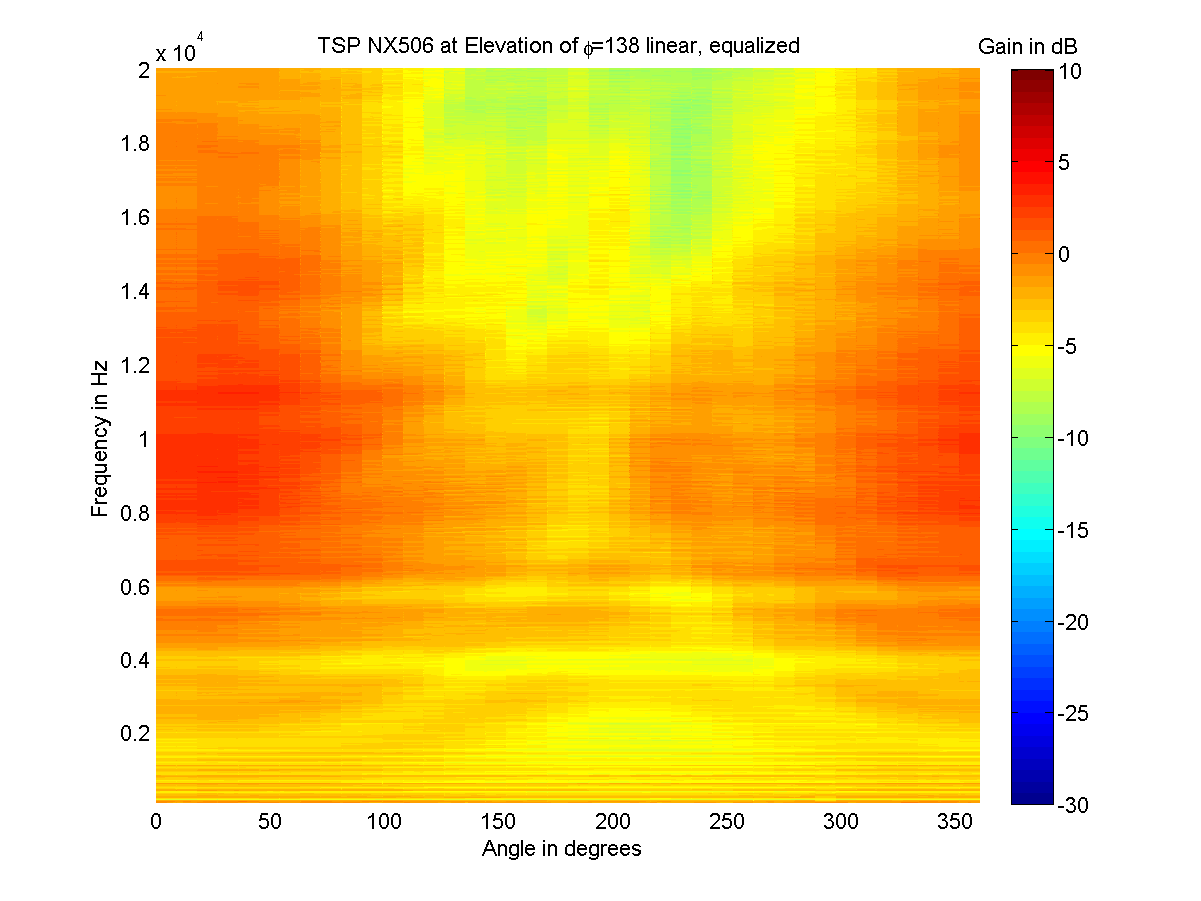
\includegraphics[height=0.28\textheight]{afbeeldingen/plots/results/NX506_TSP_138_lin_eq.png}
        \end{subfigure}~
        \begin{subfigure}[t]{0.5\textwidth}
			    \caption{North pole: $\phi=0^\circ$}
			    \label{fig:res_NX506_pluis_0}
                \centering
    			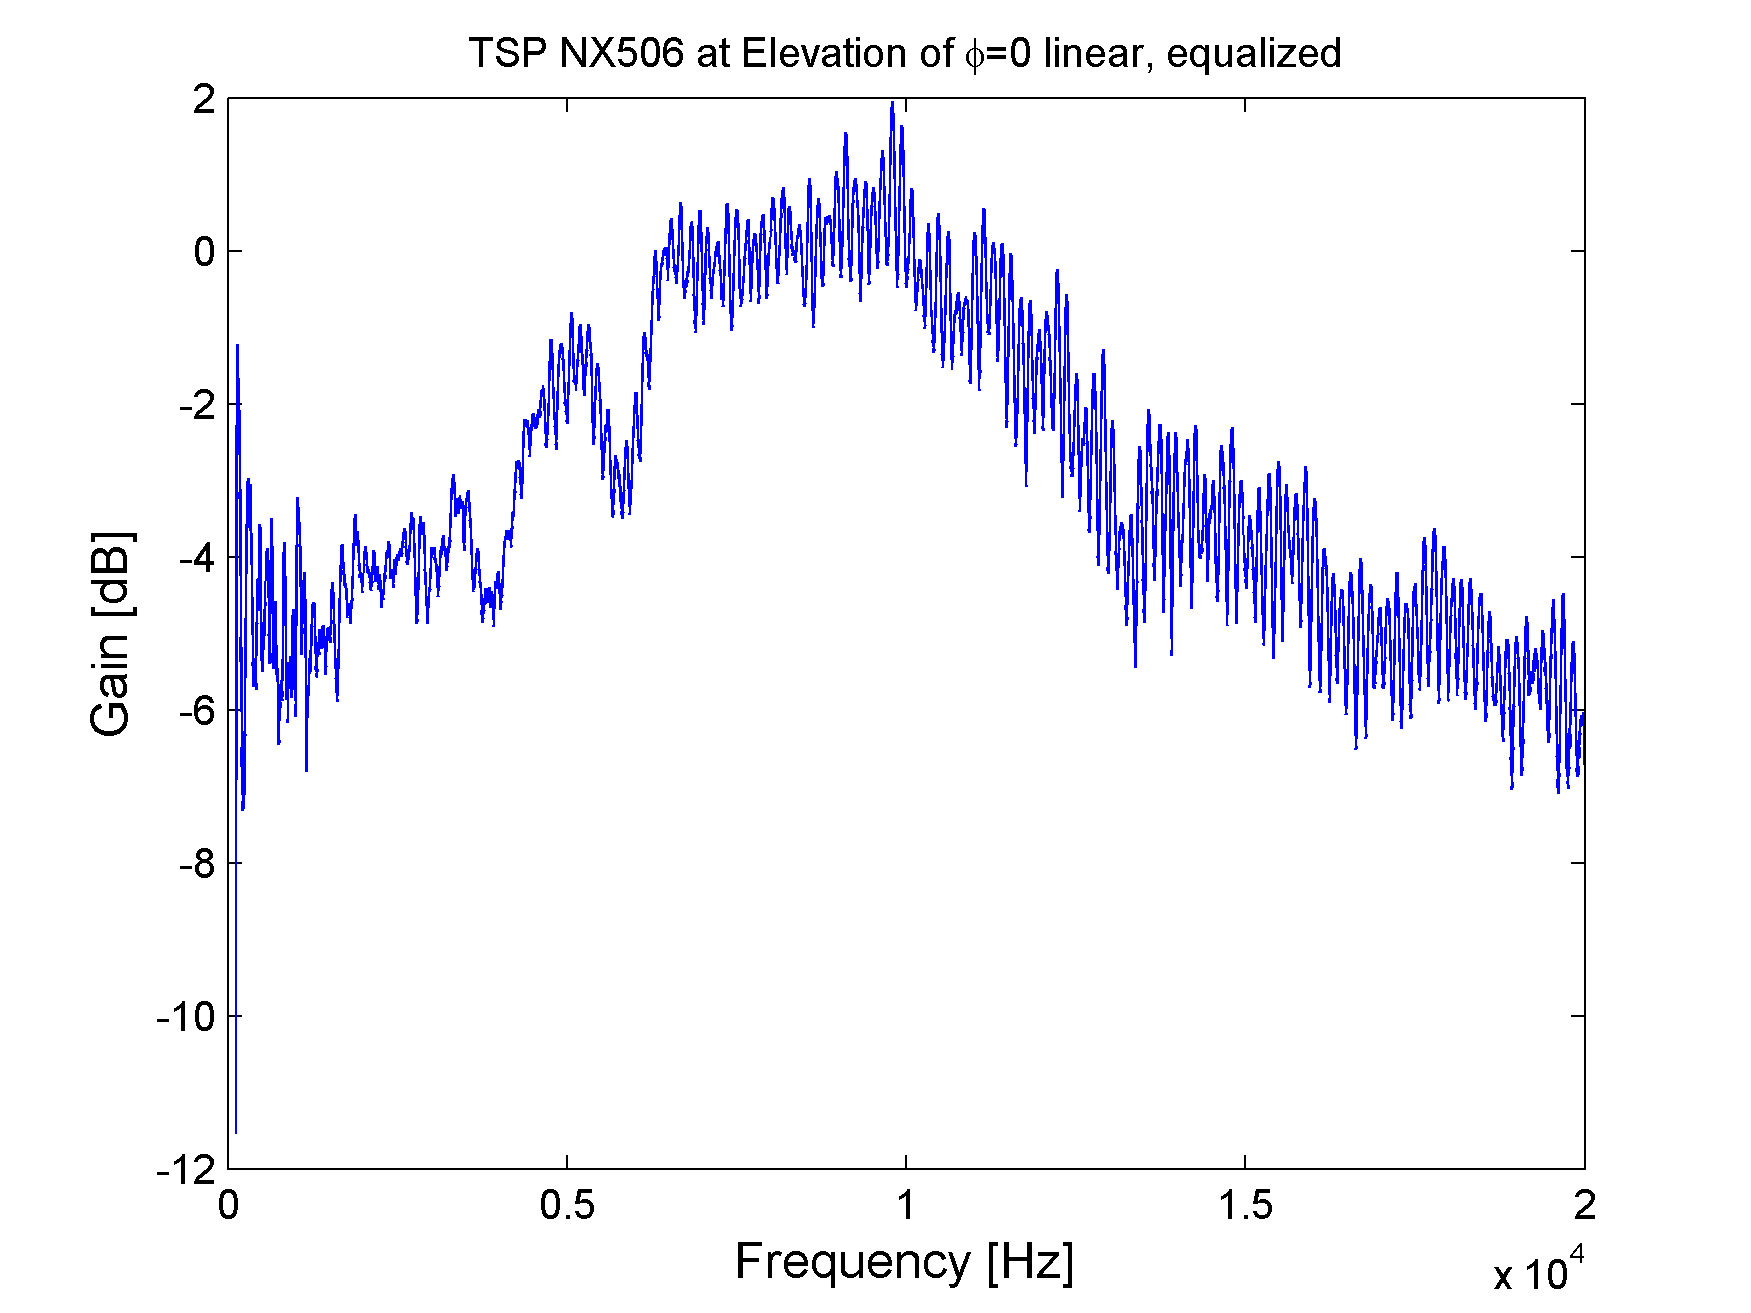
\includegraphics[height=0.28\textheight]{afbeeldingen/plots/results/NX506_north.png}
        \end{subfigure}
        
        \begin{subfigure}[t]{0.5\textwidth}
			    \caption{Full sphere $f=10000$ Hz, from the left}
			    \label{fig:res_NX506_pluis_sphere_left}
                \centering
    			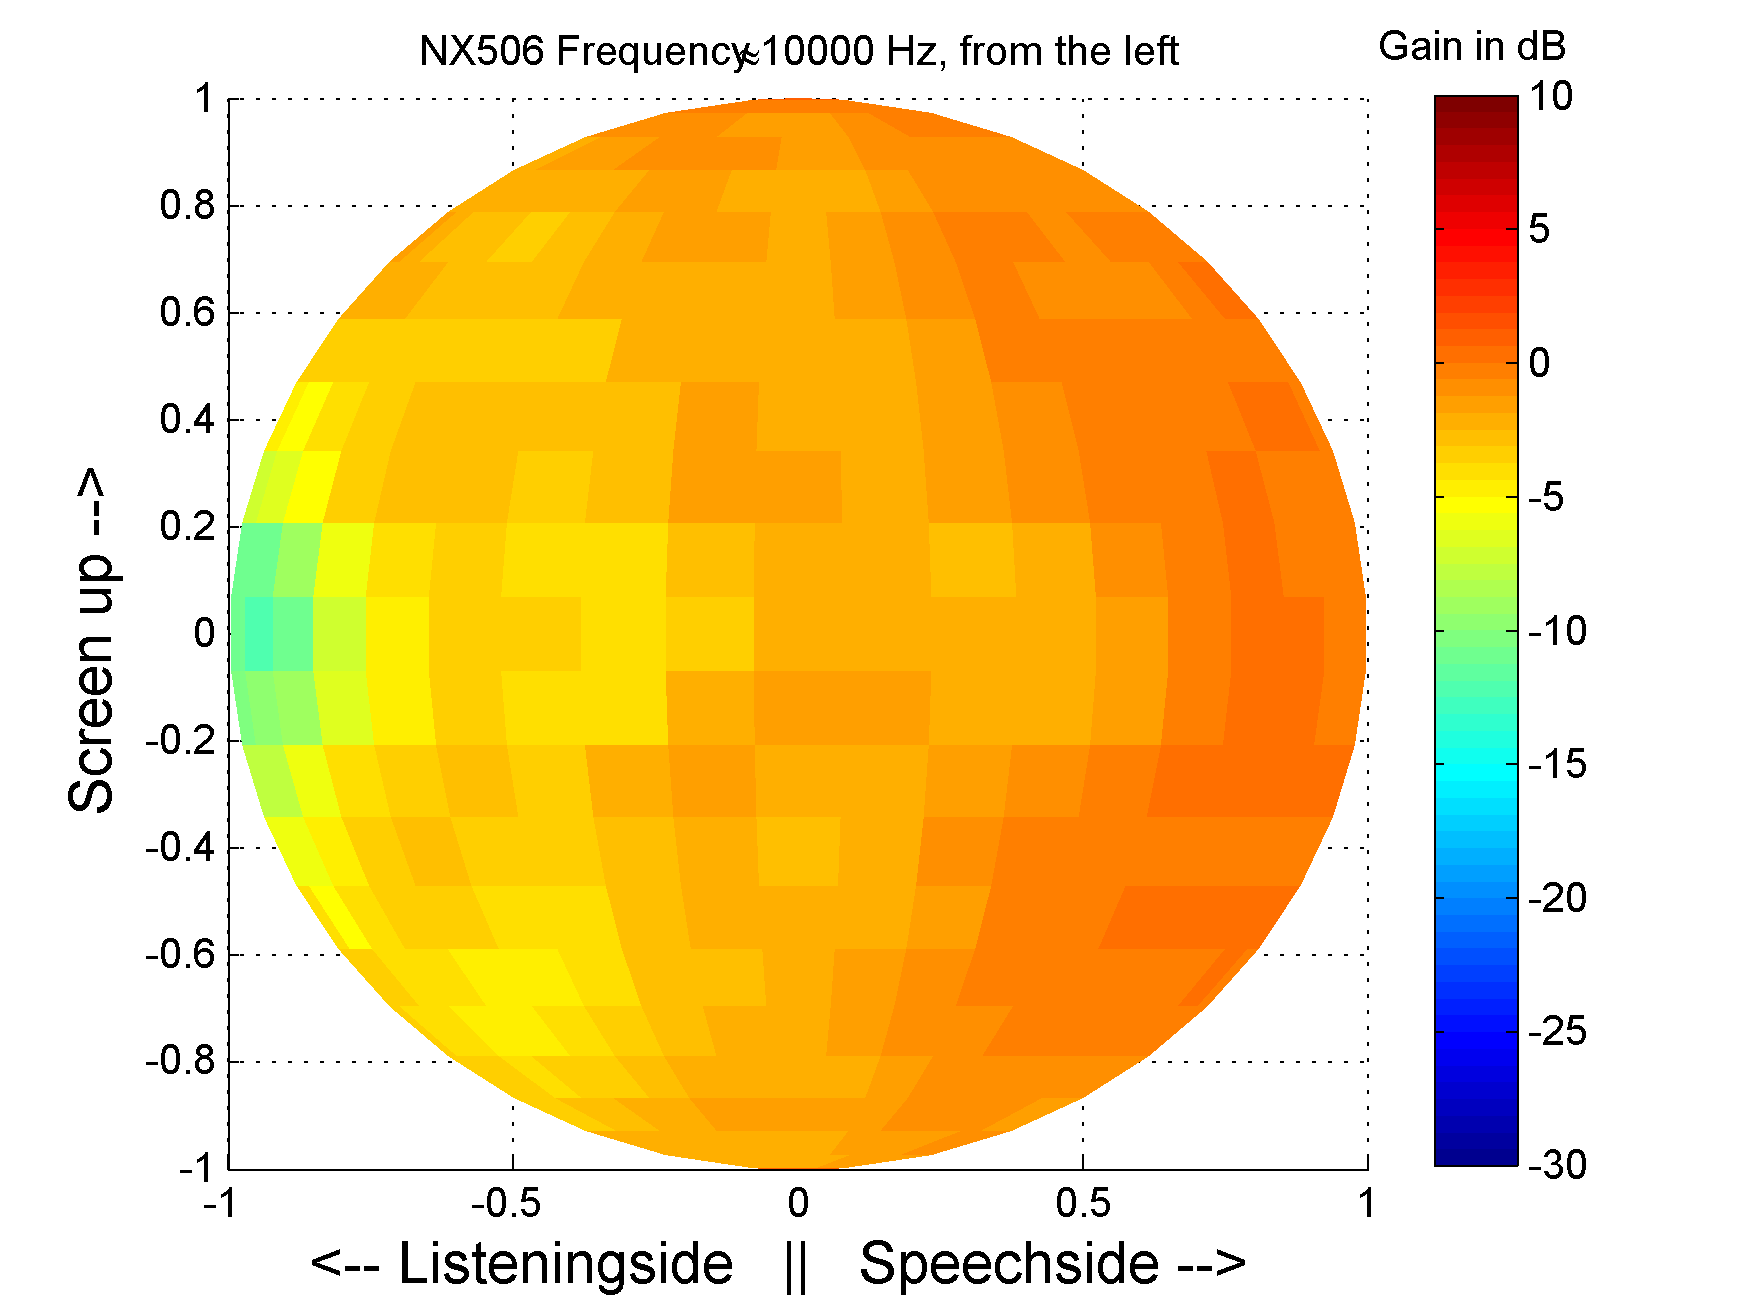
\includegraphics[height=0.28\textheight]{afbeeldingen/plots/results/NX506_10000_left.png}
        \end{subfigure}~
        \begin{subfigure}[t]{0.5\textwidth}
			    \caption{Full sphere $f=10000$ Hz, from the right}
			    \label{fig:res_NX506_pluis_sphere_right}
                \centering
    			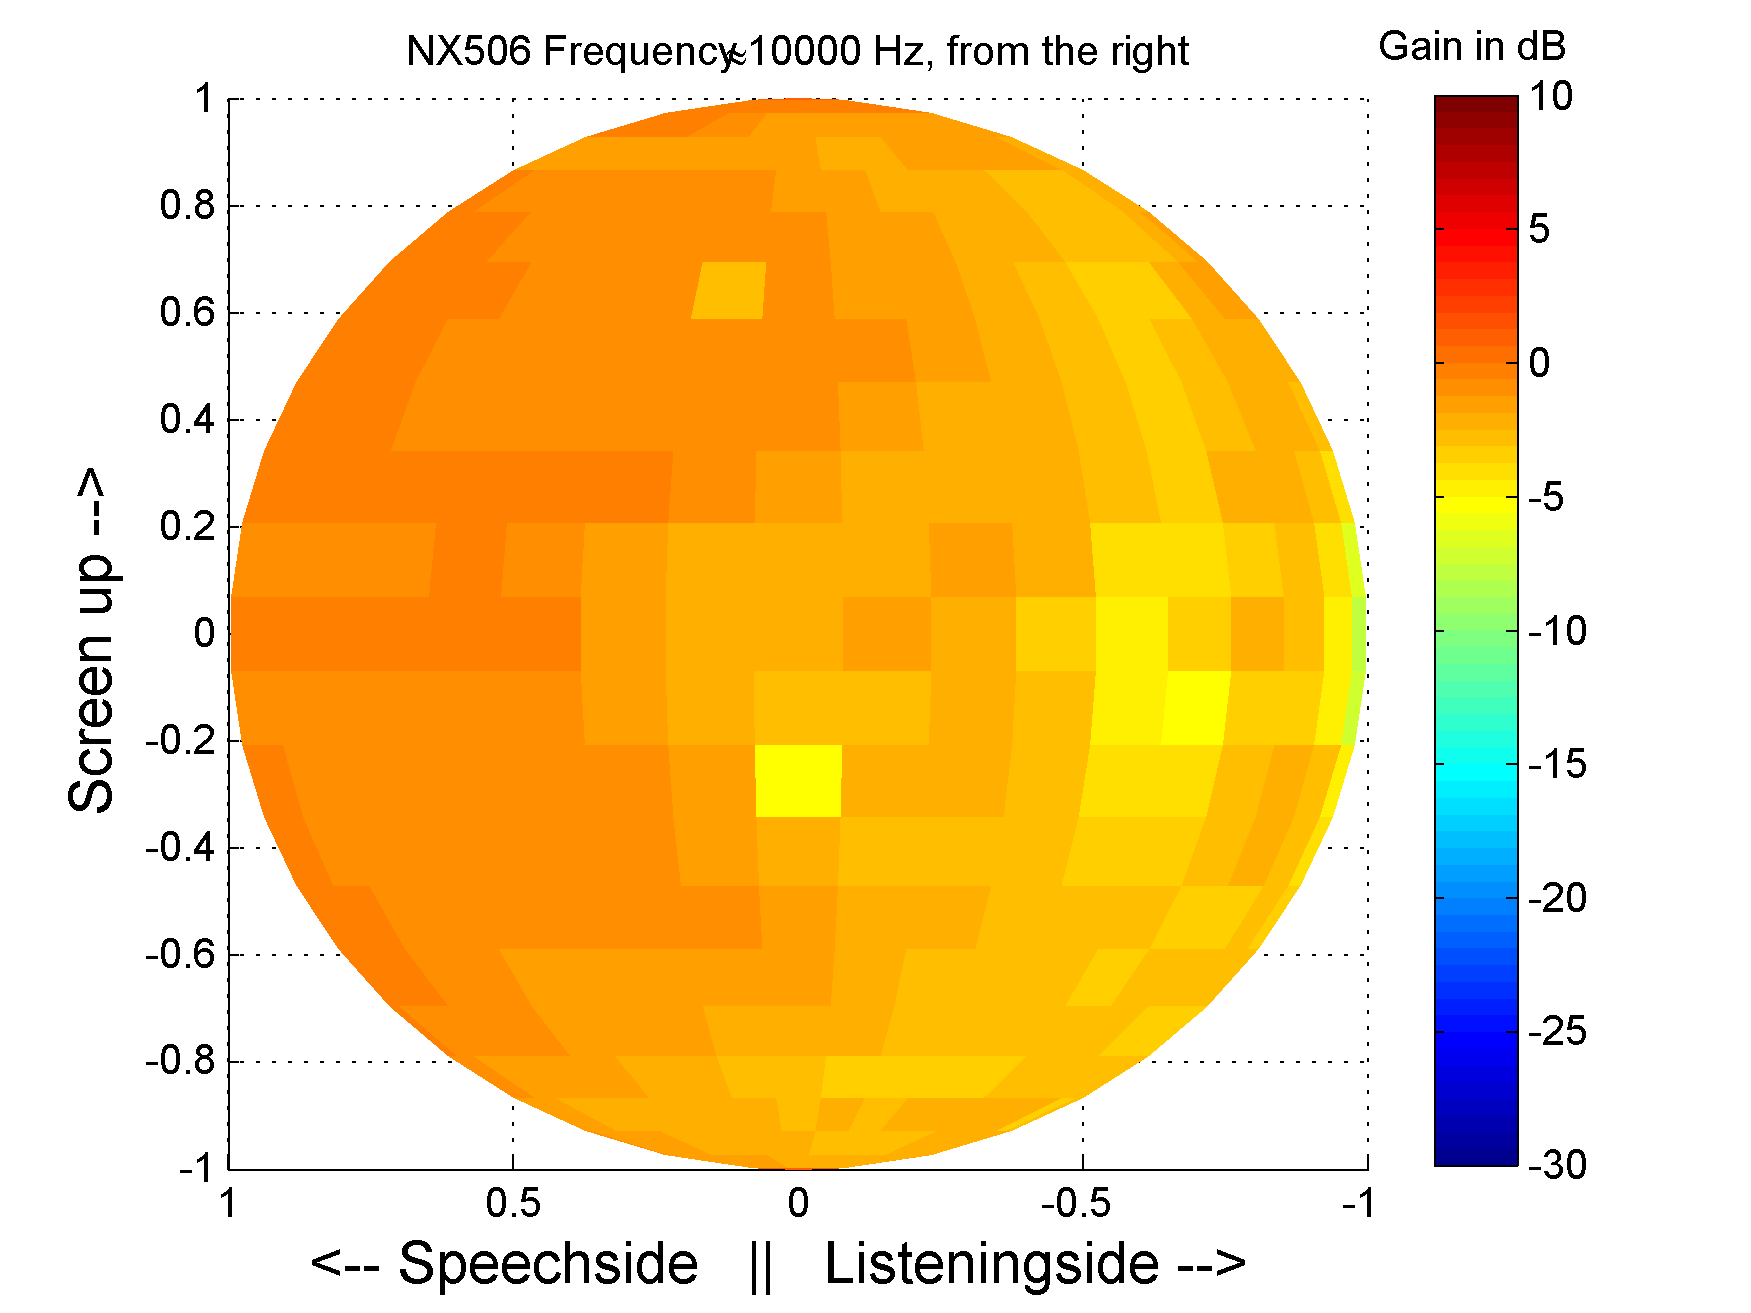
\includegraphics[height=0.28\textheight]{afbeeldingen/plots/results/NX506_10000_right.png}
        \end{subfigure}
\end{figure}

%%%%%%%%%%%%%%%%%%%%%%%%%%%%%%%%%%%%%%%%%%%%%%%%%%%%%%%%%%%%%%%%%%%%%%%%%%%%%%%%%%%%%%%%%%%%
% NX506 FU
\clearpage
\begin{figure}[t!]
        \centering
        
        \caption[Measurement results {\nexus} (6), face up]{{\nexus}, labelled with number 6, measurements in face up position, equalized}
        \label{fig:res_NX506_FU}

        \begin{subfigure}[t]{0.5\textwidth}
			    \caption{$\phi=90^\circ$}
			    \label{fig:res_NX506_FU_90}
                \centering
    			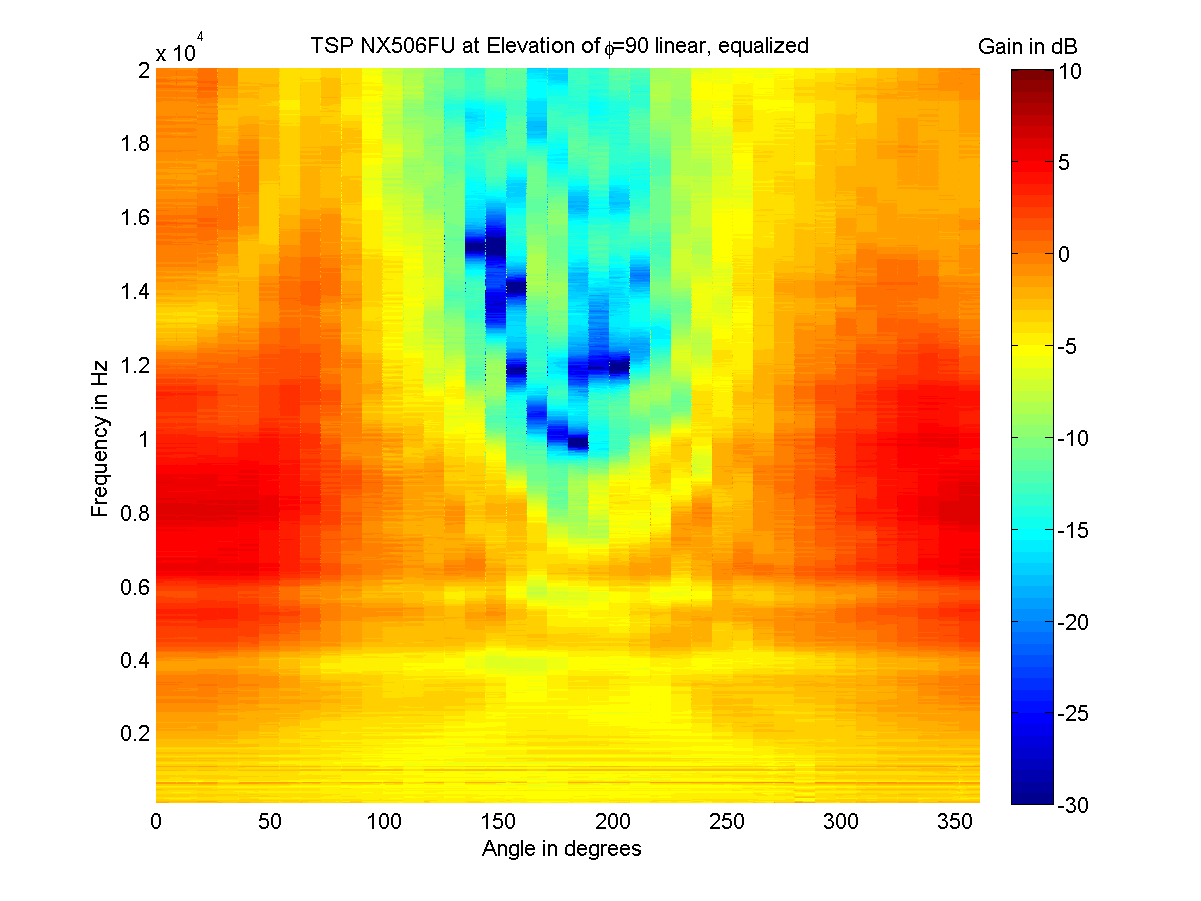
\includegraphics[height=0.28\textheight]{afbeeldingen/plots/results/NX506FU_TSP_090_lin_eq.png}
        \end{subfigure}~
        \begin{subfigure}[t]{0.5\textwidth}
			    \caption{$\phi=45^\circ$}
			    \label{fig:res_NX506_FU_45}
                \centering
    			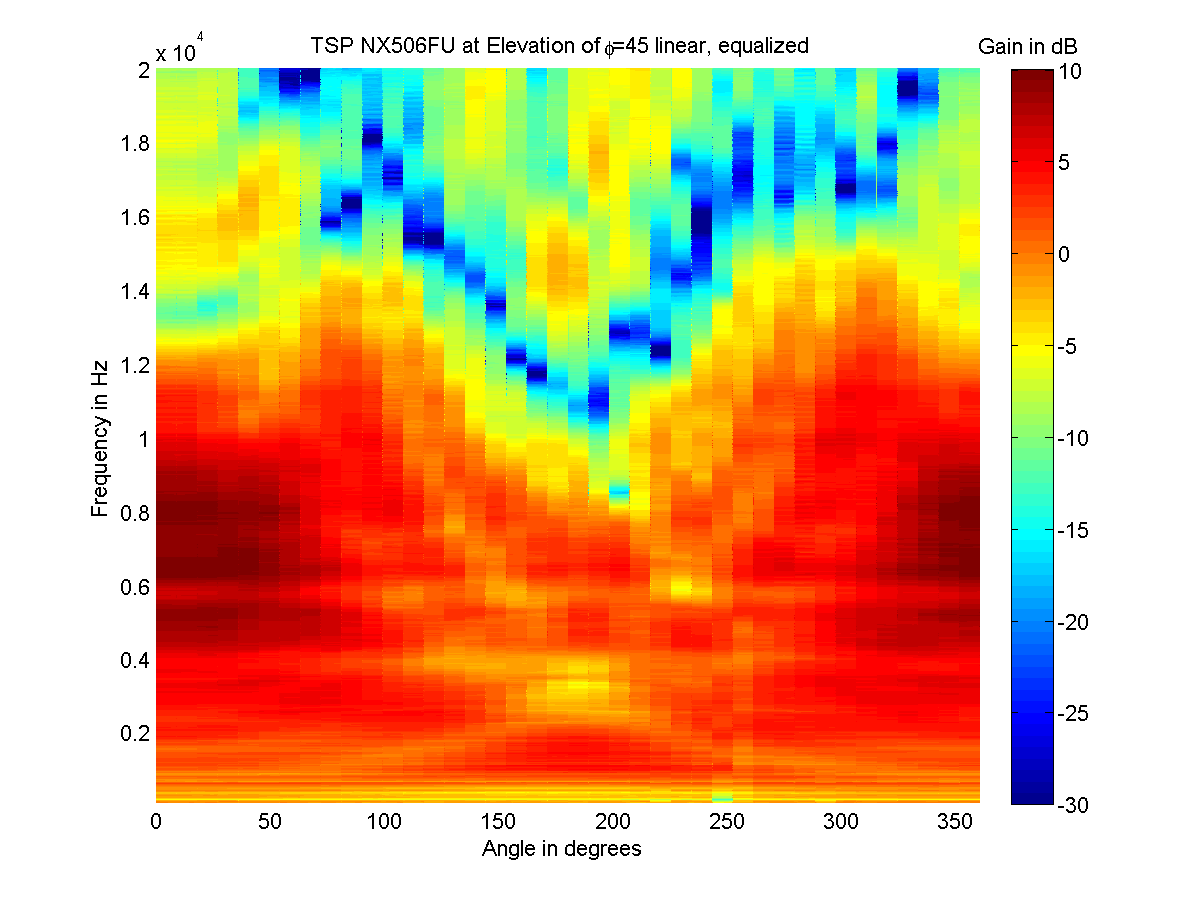
\includegraphics[height=0.28\textheight]{afbeeldingen/plots/results/NX506FU_TSP_045_lin_eq.png}
        \end{subfigure}
        
        \begin{subfigure}[t]{0.5\textwidth}
			    \caption{$\phi=135^\circ$}
			    \label{fig:res_NX506_FU_135}
                \centering
    			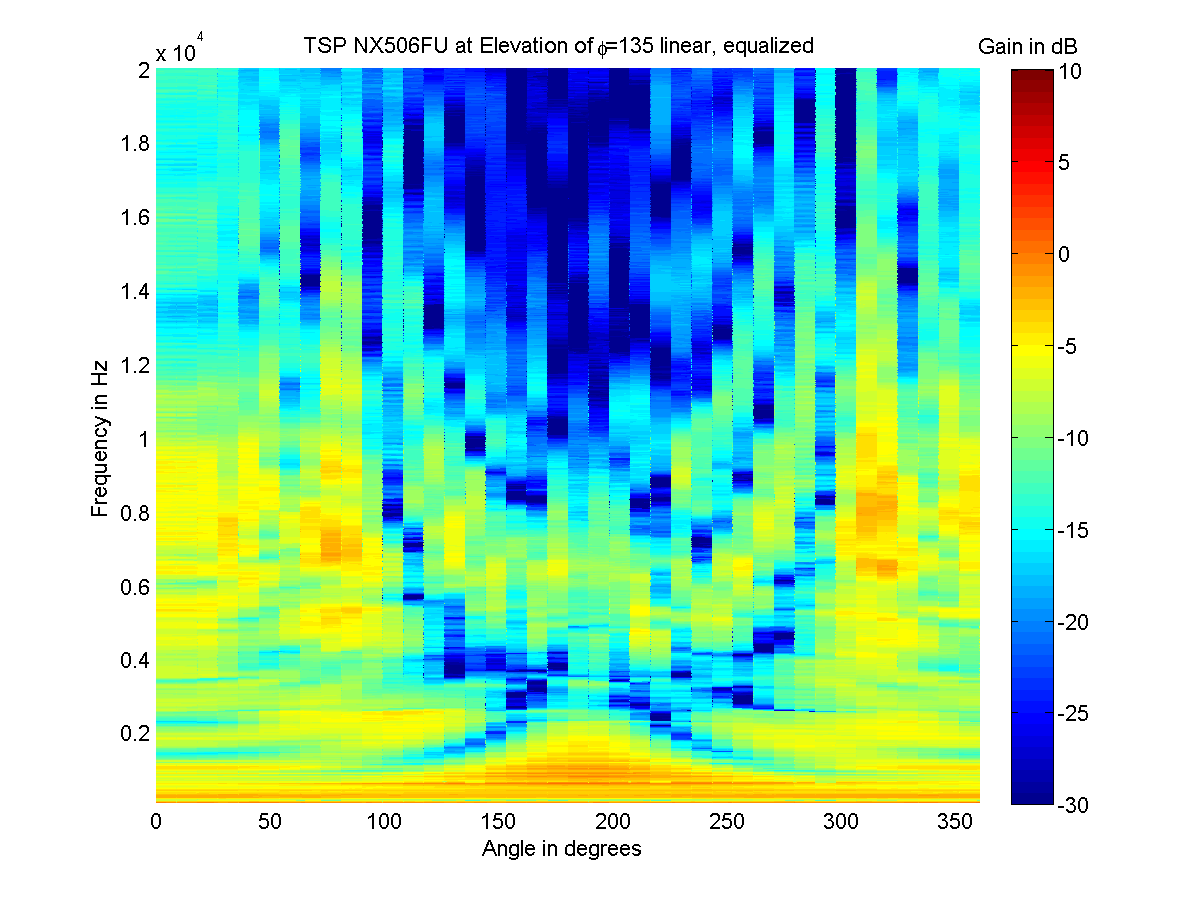
\includegraphics[height=0.28\textheight]{afbeeldingen/plots/results/NX506FU_TSP_135_lin_eq.png}
        \end{subfigure}~
        \begin{subfigure}[t]{0.5\textwidth}
			    \caption{North pole: $\phi=0^\circ$}
			    \label{fig:res_NX506_FU_0}
                \centering
    			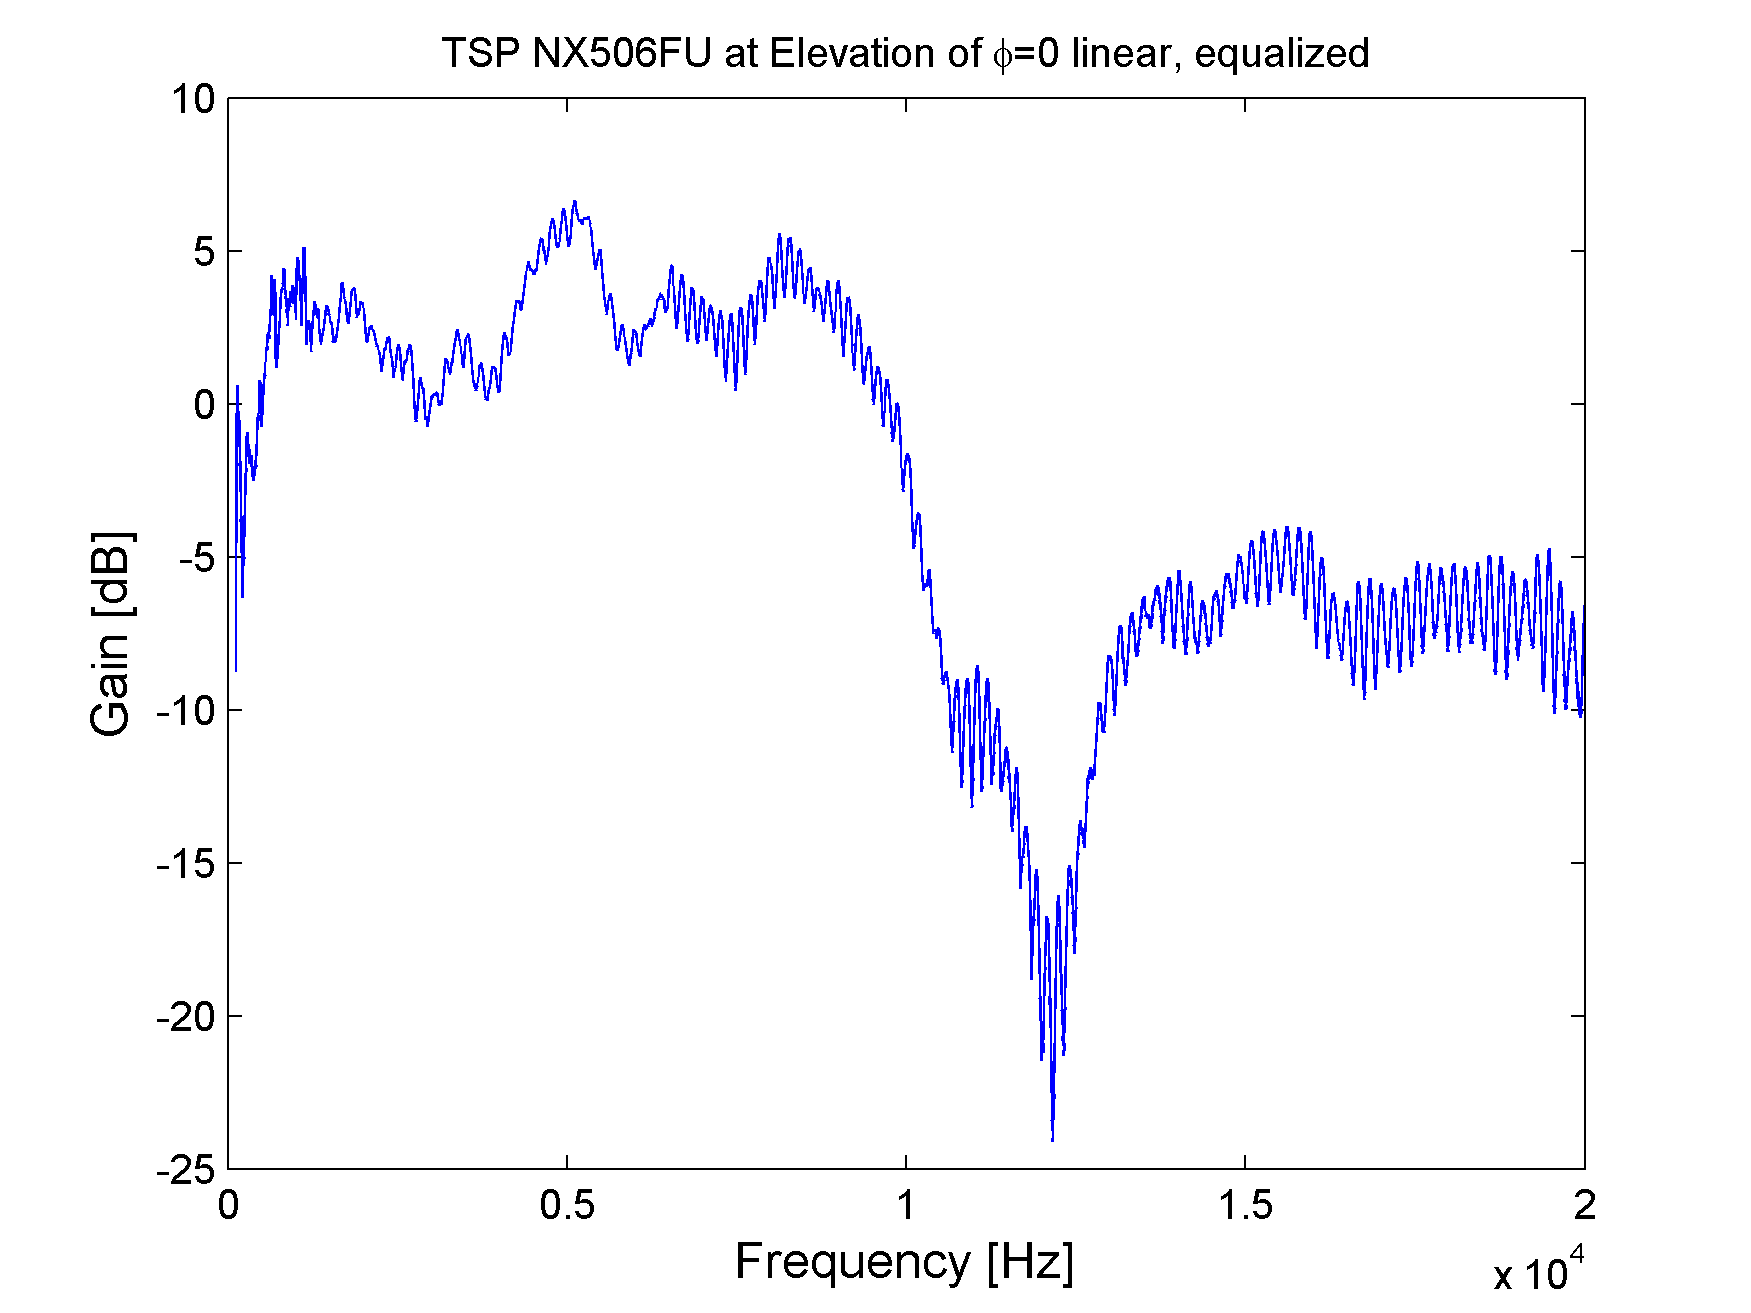
\includegraphics[height=0.28\textheight]{afbeeldingen/plots/results/NX506FU_north.png}
        \end{subfigure}
        
        \begin{subfigure}[t]{0.5\textwidth}
			    \caption{Full sphere $f=10000$ Hz, from the left}
			    \label{fig:res_NX506_FU_sphere_left}
                \centering
    			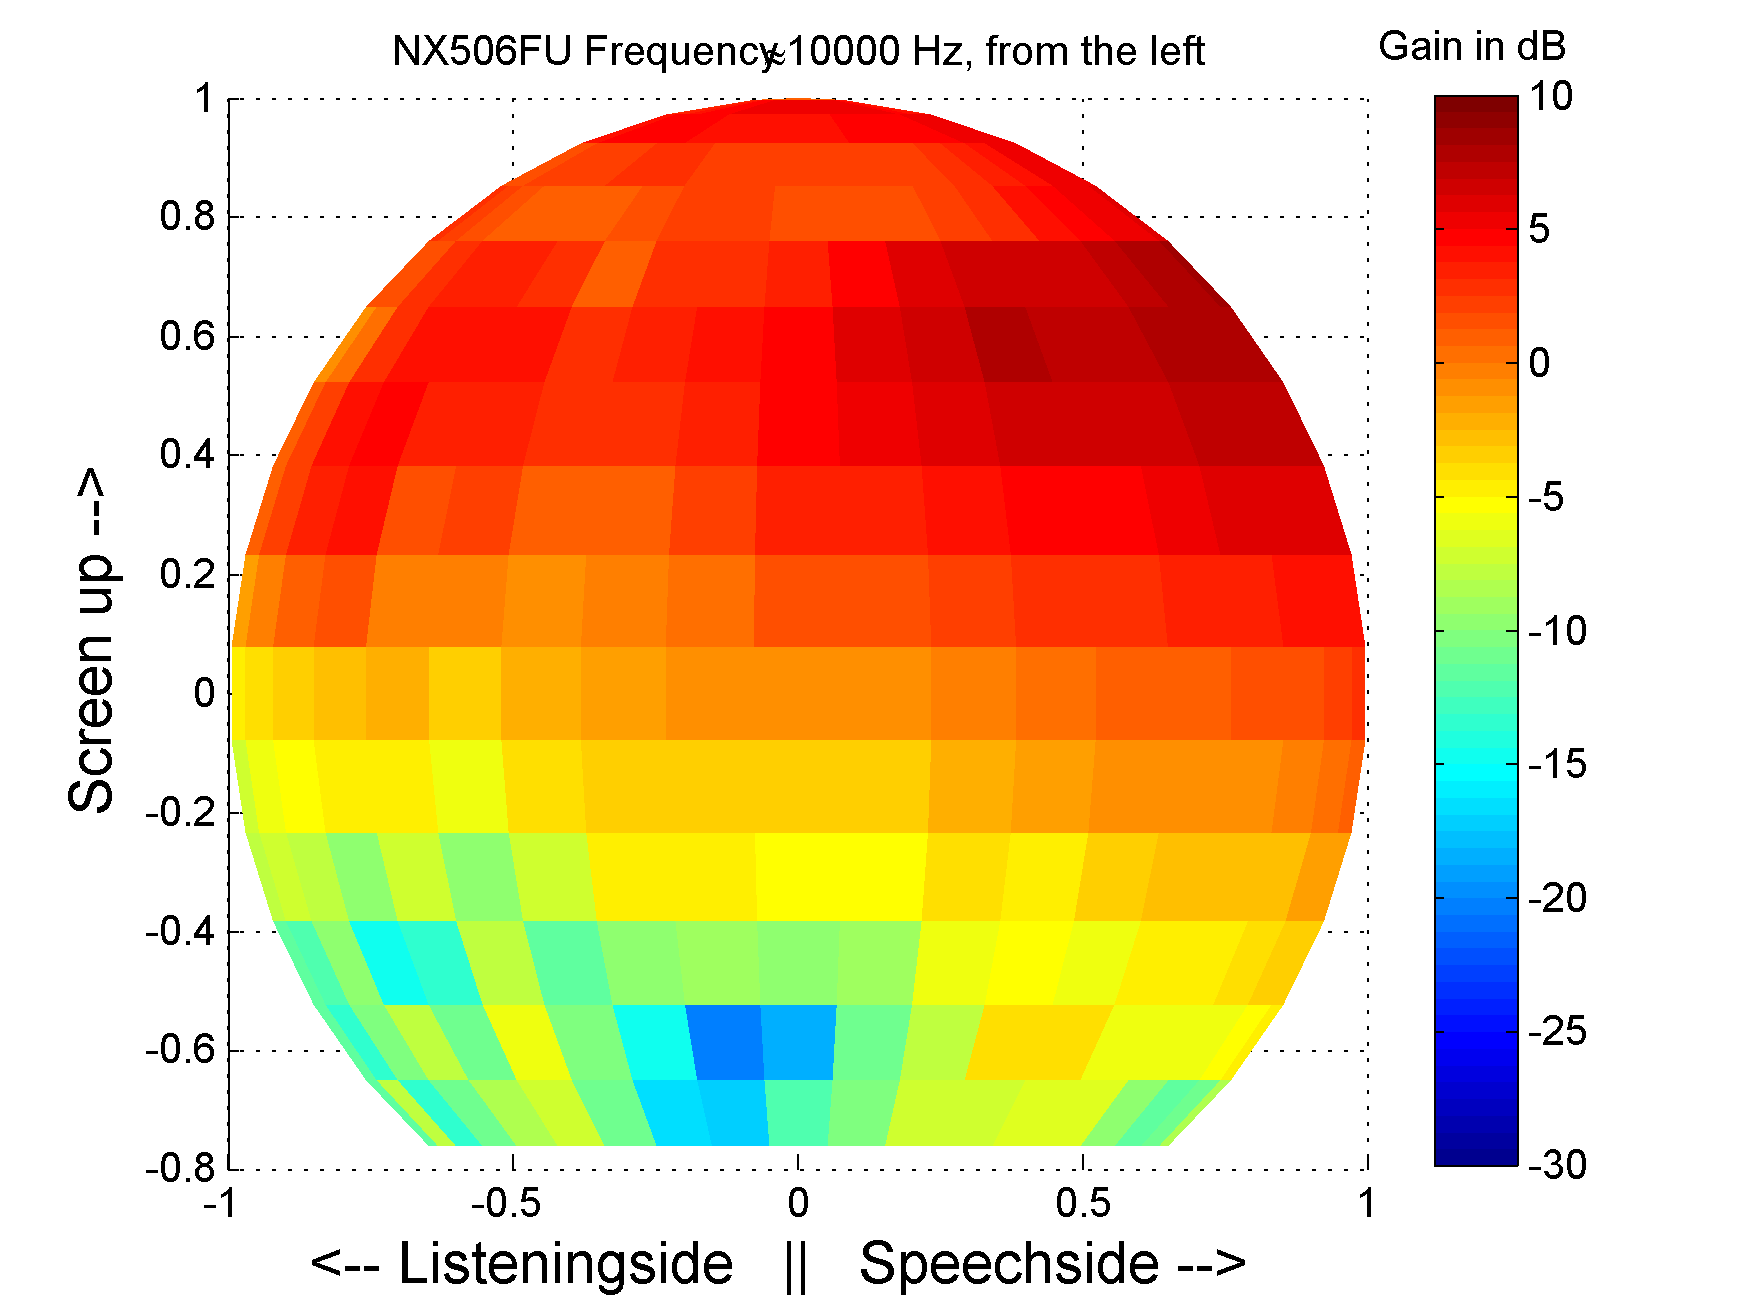
\includegraphics[height=0.28\textheight]{afbeeldingen/plots/results/NX506FU_10000_left.png}
        \end{subfigure}~
        \begin{subfigure}[t]{0.5\textwidth}
			    \caption{Full sphere $f=10000$ Hz, from the right}
			    \label{fig:res_NX506_FU_sphere_right}
                \centering
    			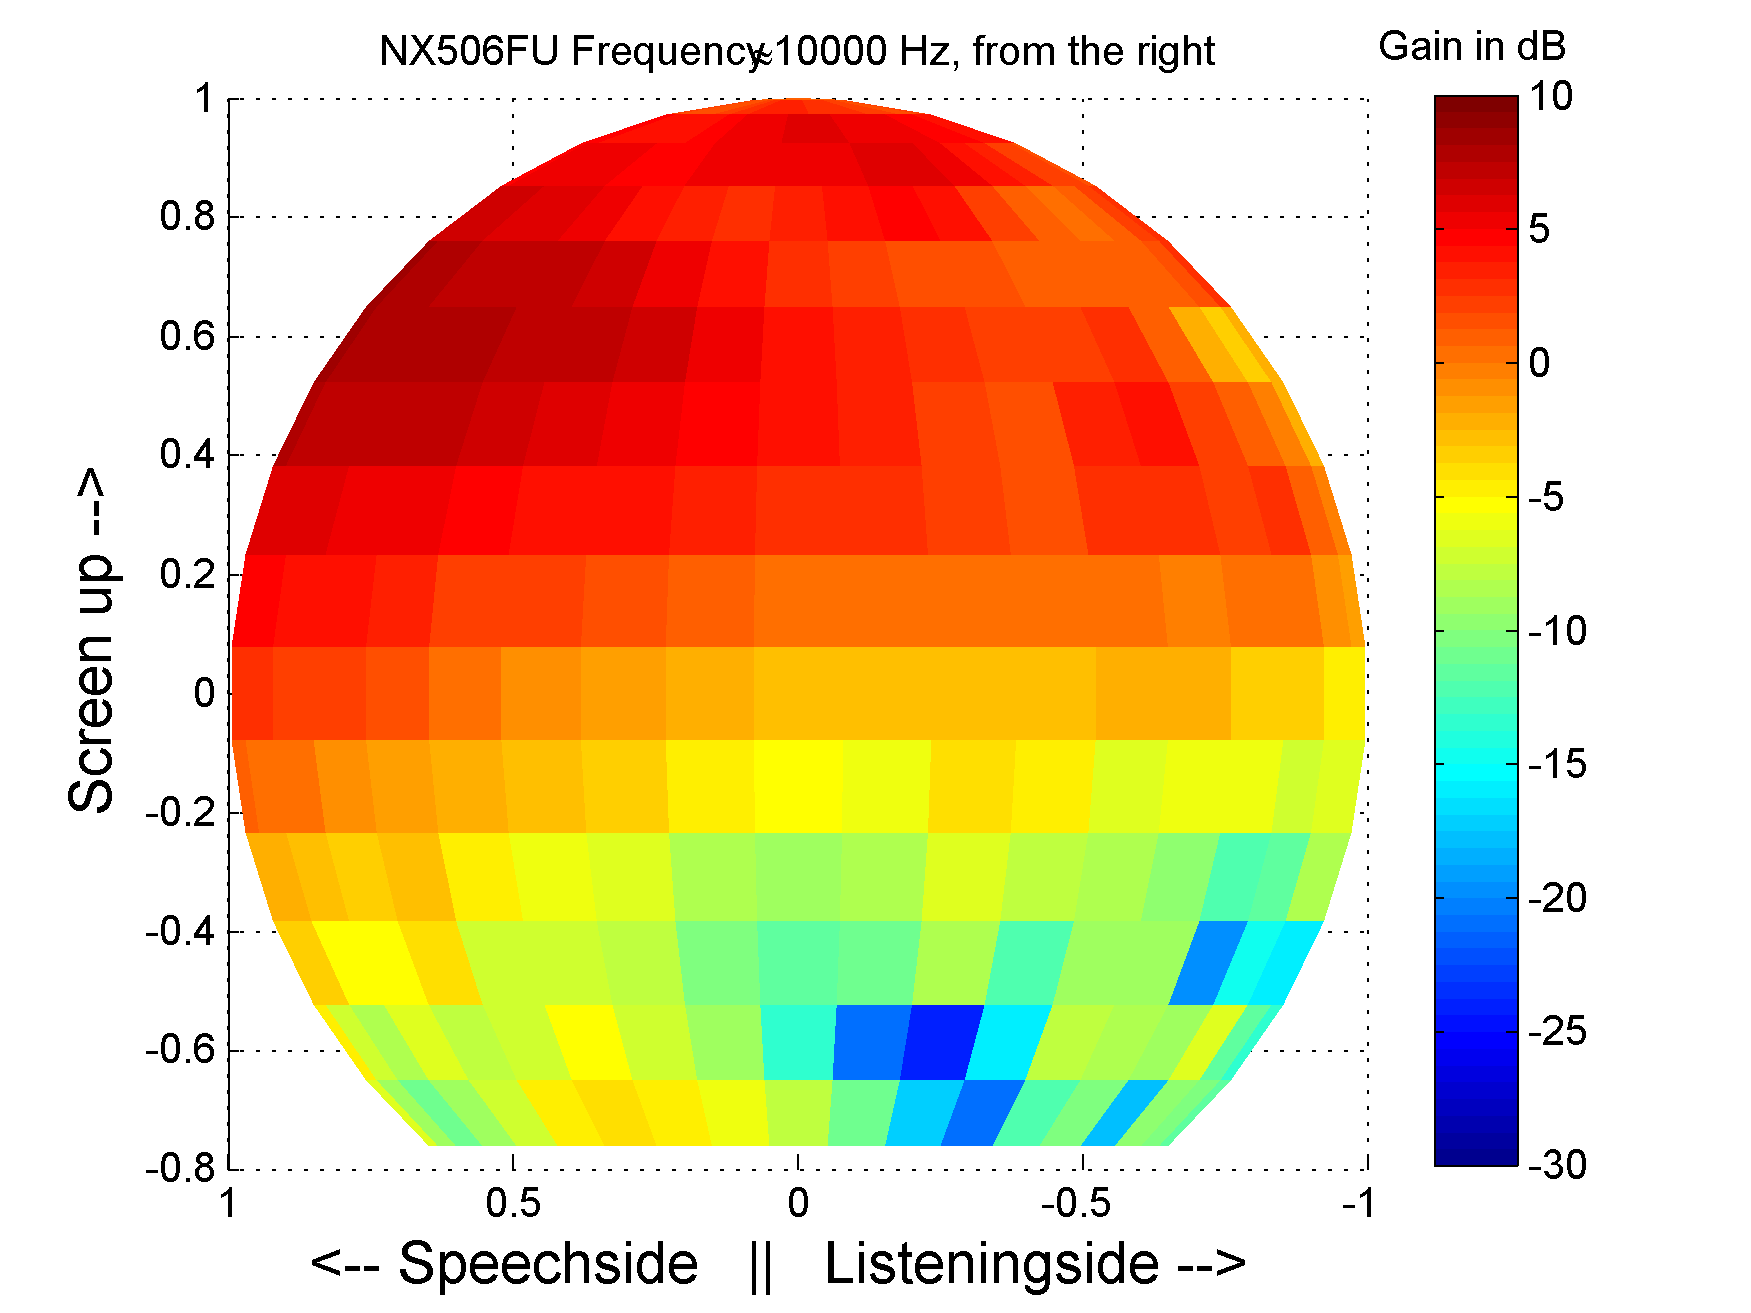
\includegraphics[height=0.28\textheight]{afbeeldingen/plots/results/NX506FU_10000_right.png}
        \end{subfigure}
\end{figure}

%%%%%%%%%%%%%%%%%%%%%%%%%%%%%%%%%%%%%%%%%%%%%%%%%%%%%%%%%%%%%%%%%%%%%%%%%%%%%%%%%%%%%%%%%%%%
% NX506 FD
\clearpage
\begin{figure}[t!]
        \centering
        
        \caption[Measurement results {\nexus} (6), face down]{{\nexus}, labelled with number 6, measurements in face down position, equalized}
        \label{fig:res_NX506_FD}

        \begin{subfigure}[t]{0.5\textwidth}
			    \caption{$\phi=90^\circ$}
			    \label{fig:res_NX506_FD_90}
                \centering
    			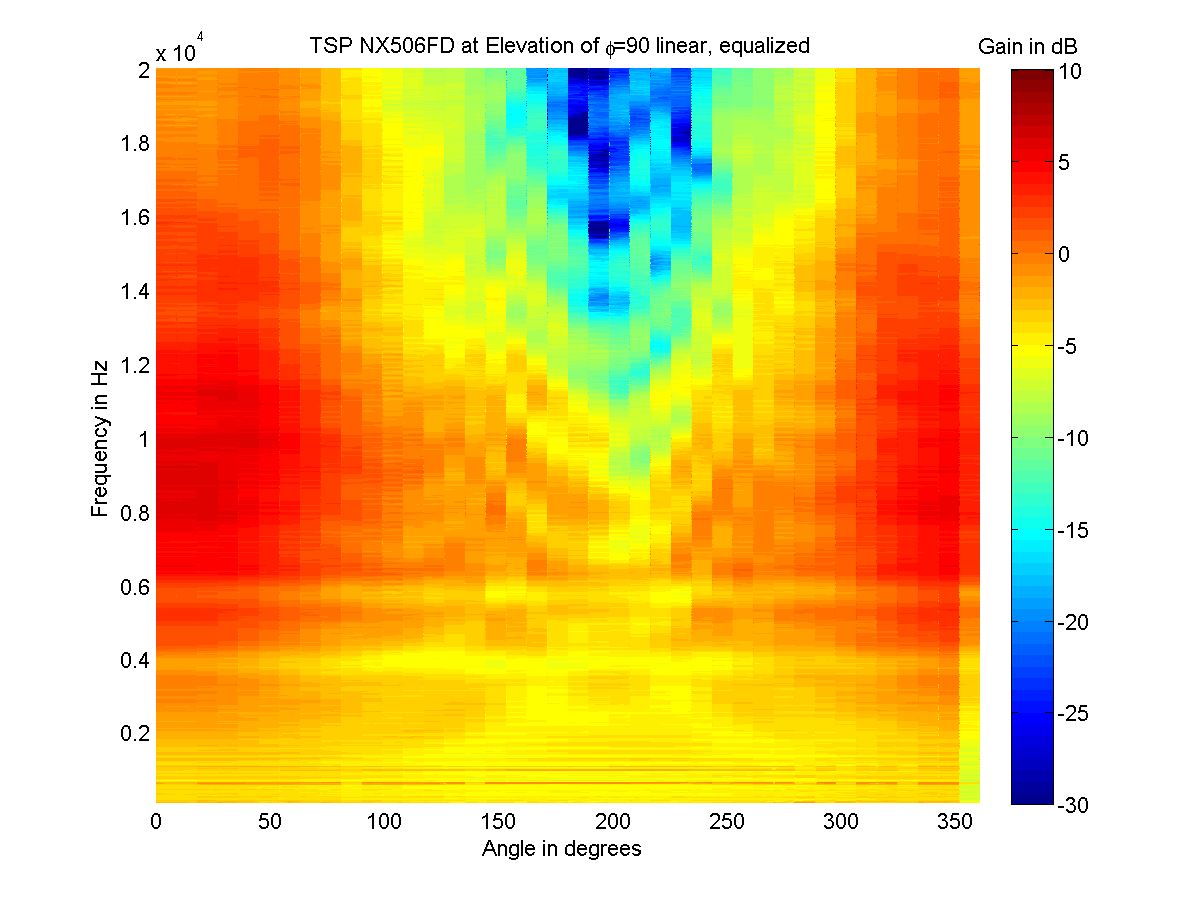
\includegraphics[height=0.28\textheight]{afbeeldingen/plots/results/NX506FD_TSP_090_lin_eq.png}
        \end{subfigure}~
        \begin{subfigure}[t]{0.5\textwidth}
			    \caption{$\phi=45^\circ$}
			    \label{fig:res_NX506_FD_45}
                \centering
    			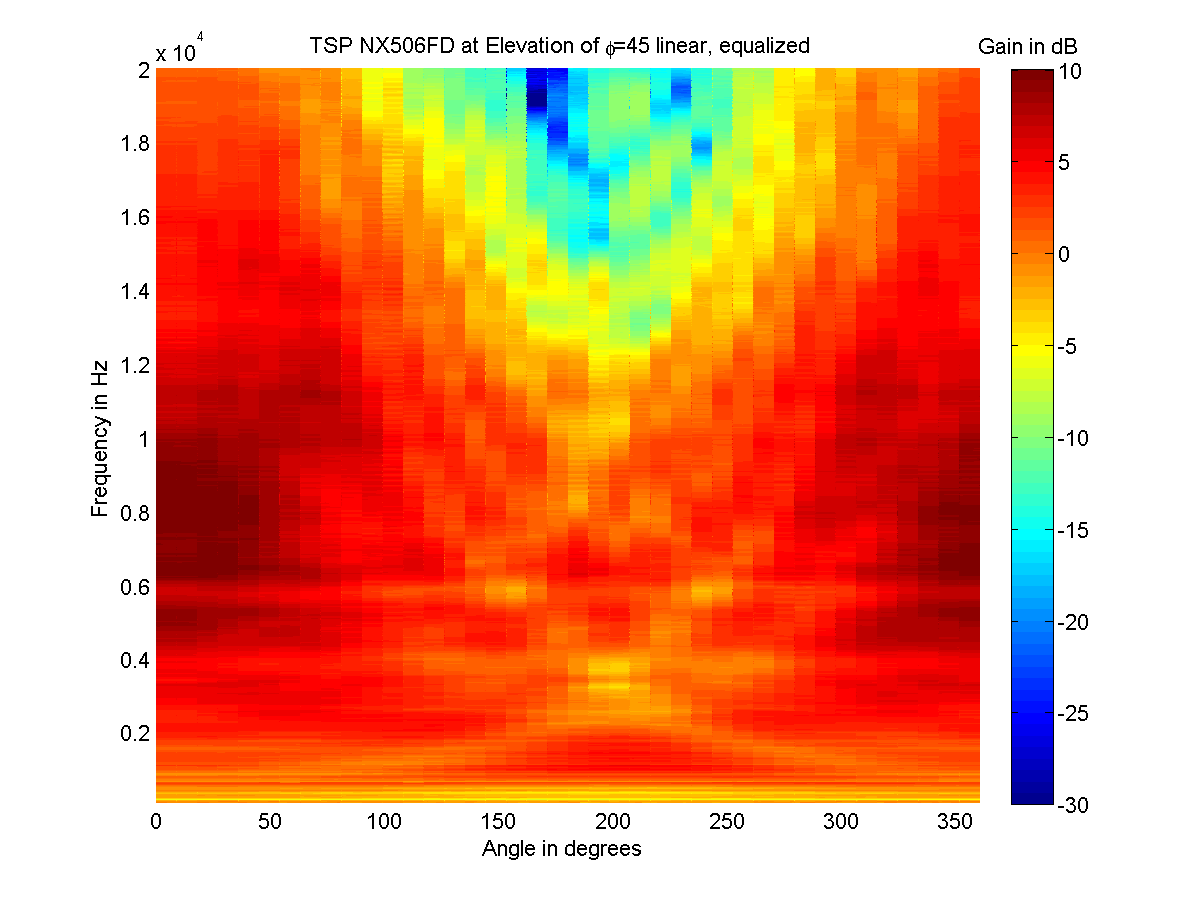
\includegraphics[height=0.28\textheight]{afbeeldingen/plots/results/NX506FD_TSP_045_lin_eq.png}
        \end{subfigure}
        
        \begin{subfigure}[t]{0.5\textwidth}
			    \caption{$\phi=135^\circ$}
			    \label{fig:res_NX506_FD_135}
                \centering
    			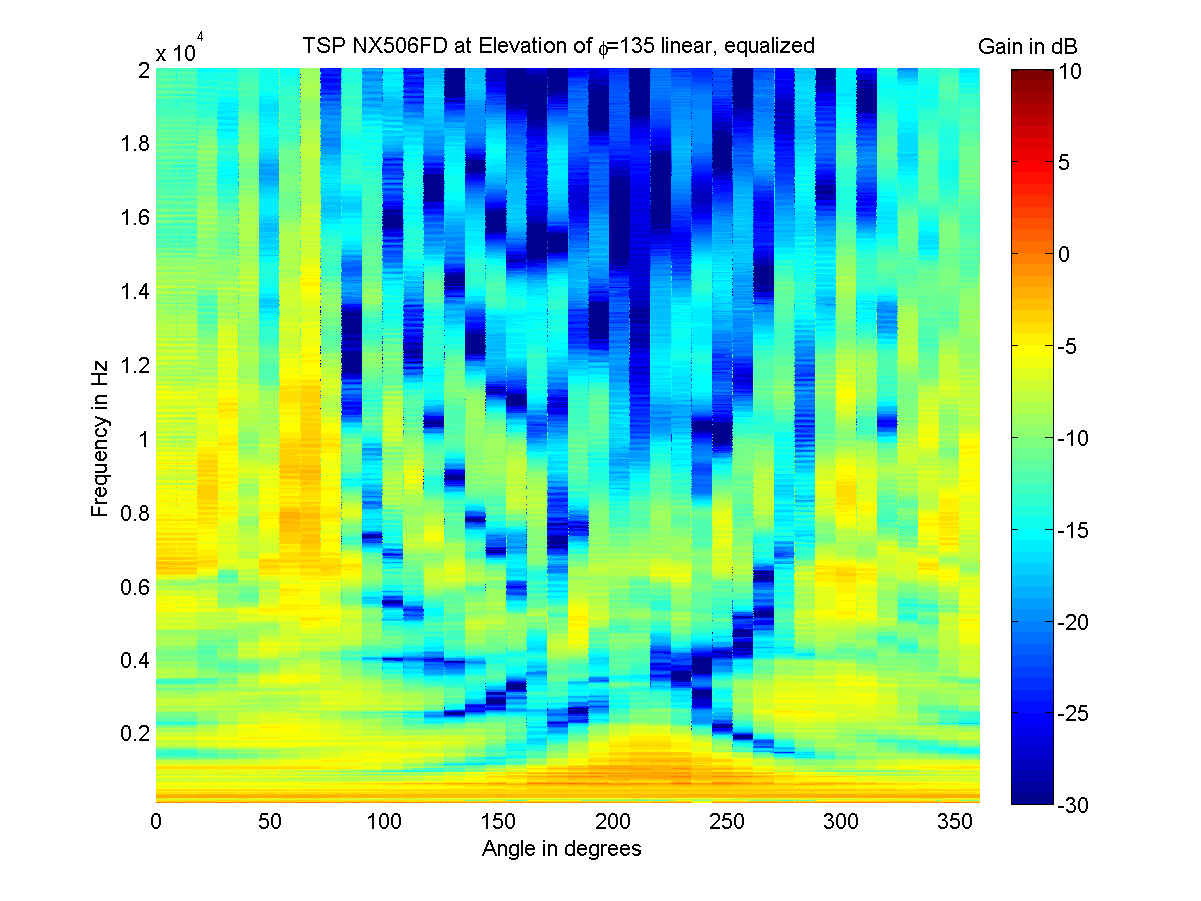
\includegraphics[height=0.28\textheight]{afbeeldingen/plots/results/NX506FD_TSP_135_lin_eq.png}
        \end{subfigure}~
        \begin{subfigure}[t]{0.5\textwidth}
			    \caption{North pole: $\phi=0^\circ$}
			    \label{fig:res_NX506_FD_0}
                \centering
    			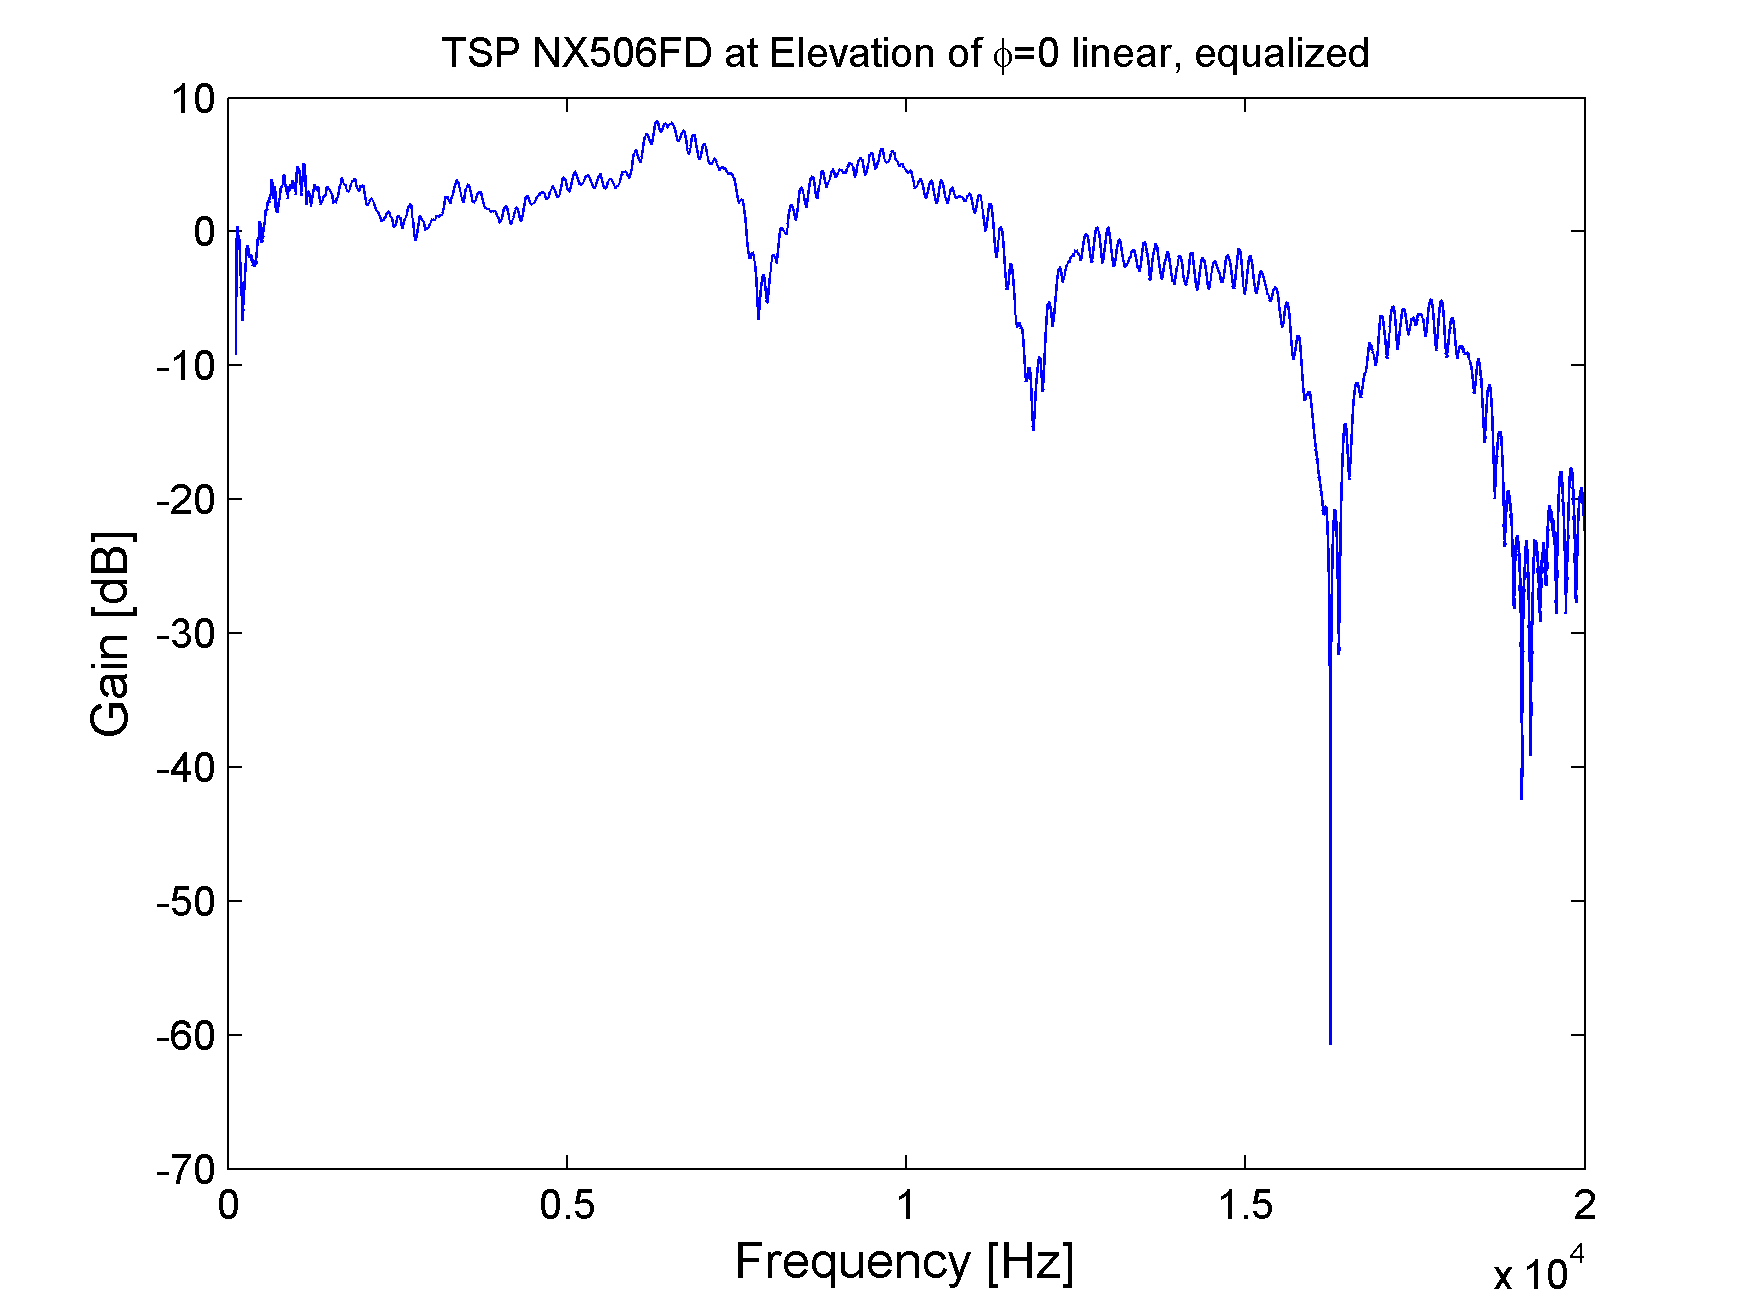
\includegraphics[height=0.28\textheight]{afbeeldingen/plots/results/NX506FD_north.png}
        \end{subfigure}
        
        \begin{subfigure}[t]{0.5\textwidth}
			    \caption{Full sphere $f=10000$ Hz, from the left}
			    \label{fig:res_NX506_FD_sphere_left}
                \centering
    			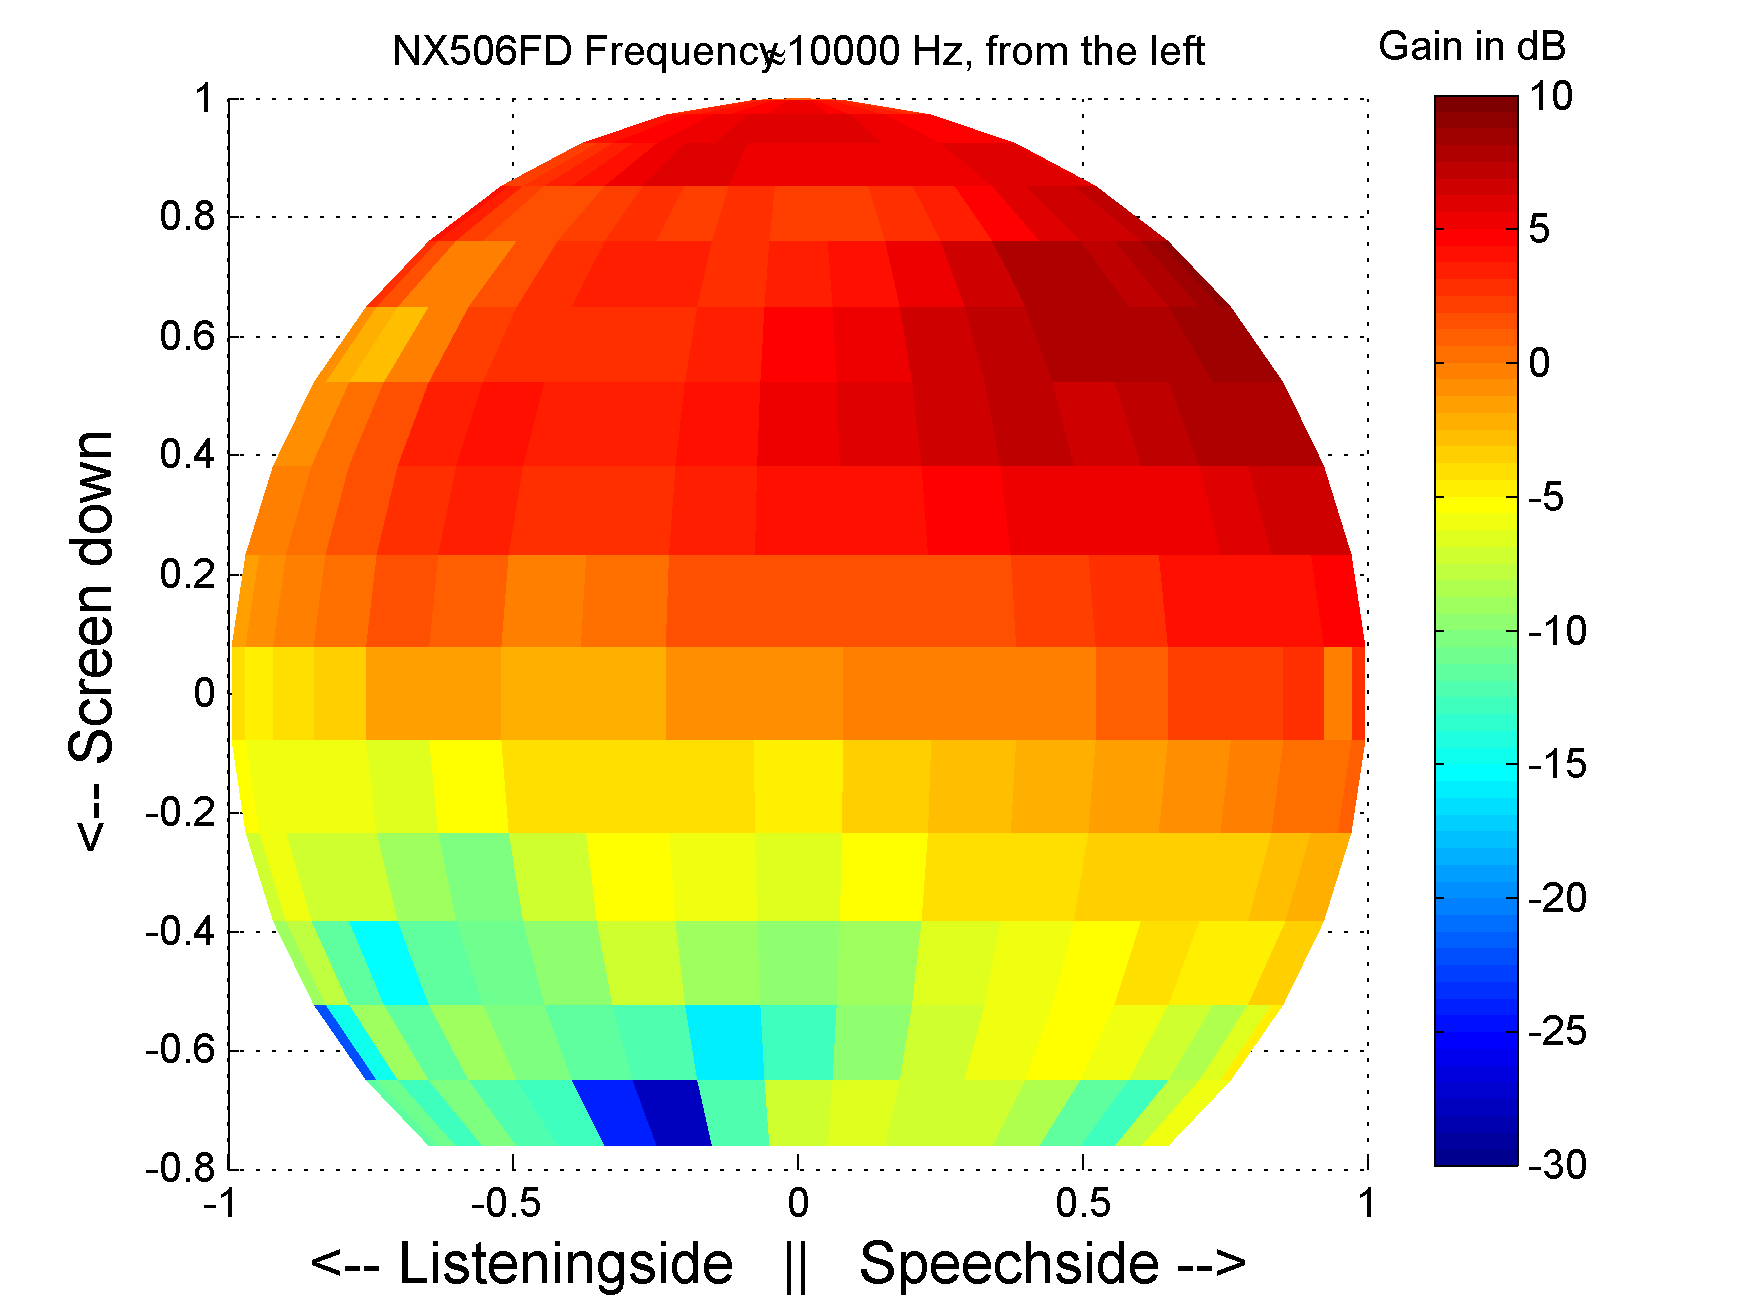
\includegraphics[height=0.28\textheight]{afbeeldingen/plots/results/NX506FD_10000_left.png}
        \end{subfigure}~
        \begin{subfigure}[t]{0.5\textwidth}
			    \caption{Full sphere $f=10000$ Hz, from the right}
			    \label{fig:res_NX506_FD_sphere_right}
                \centering
    			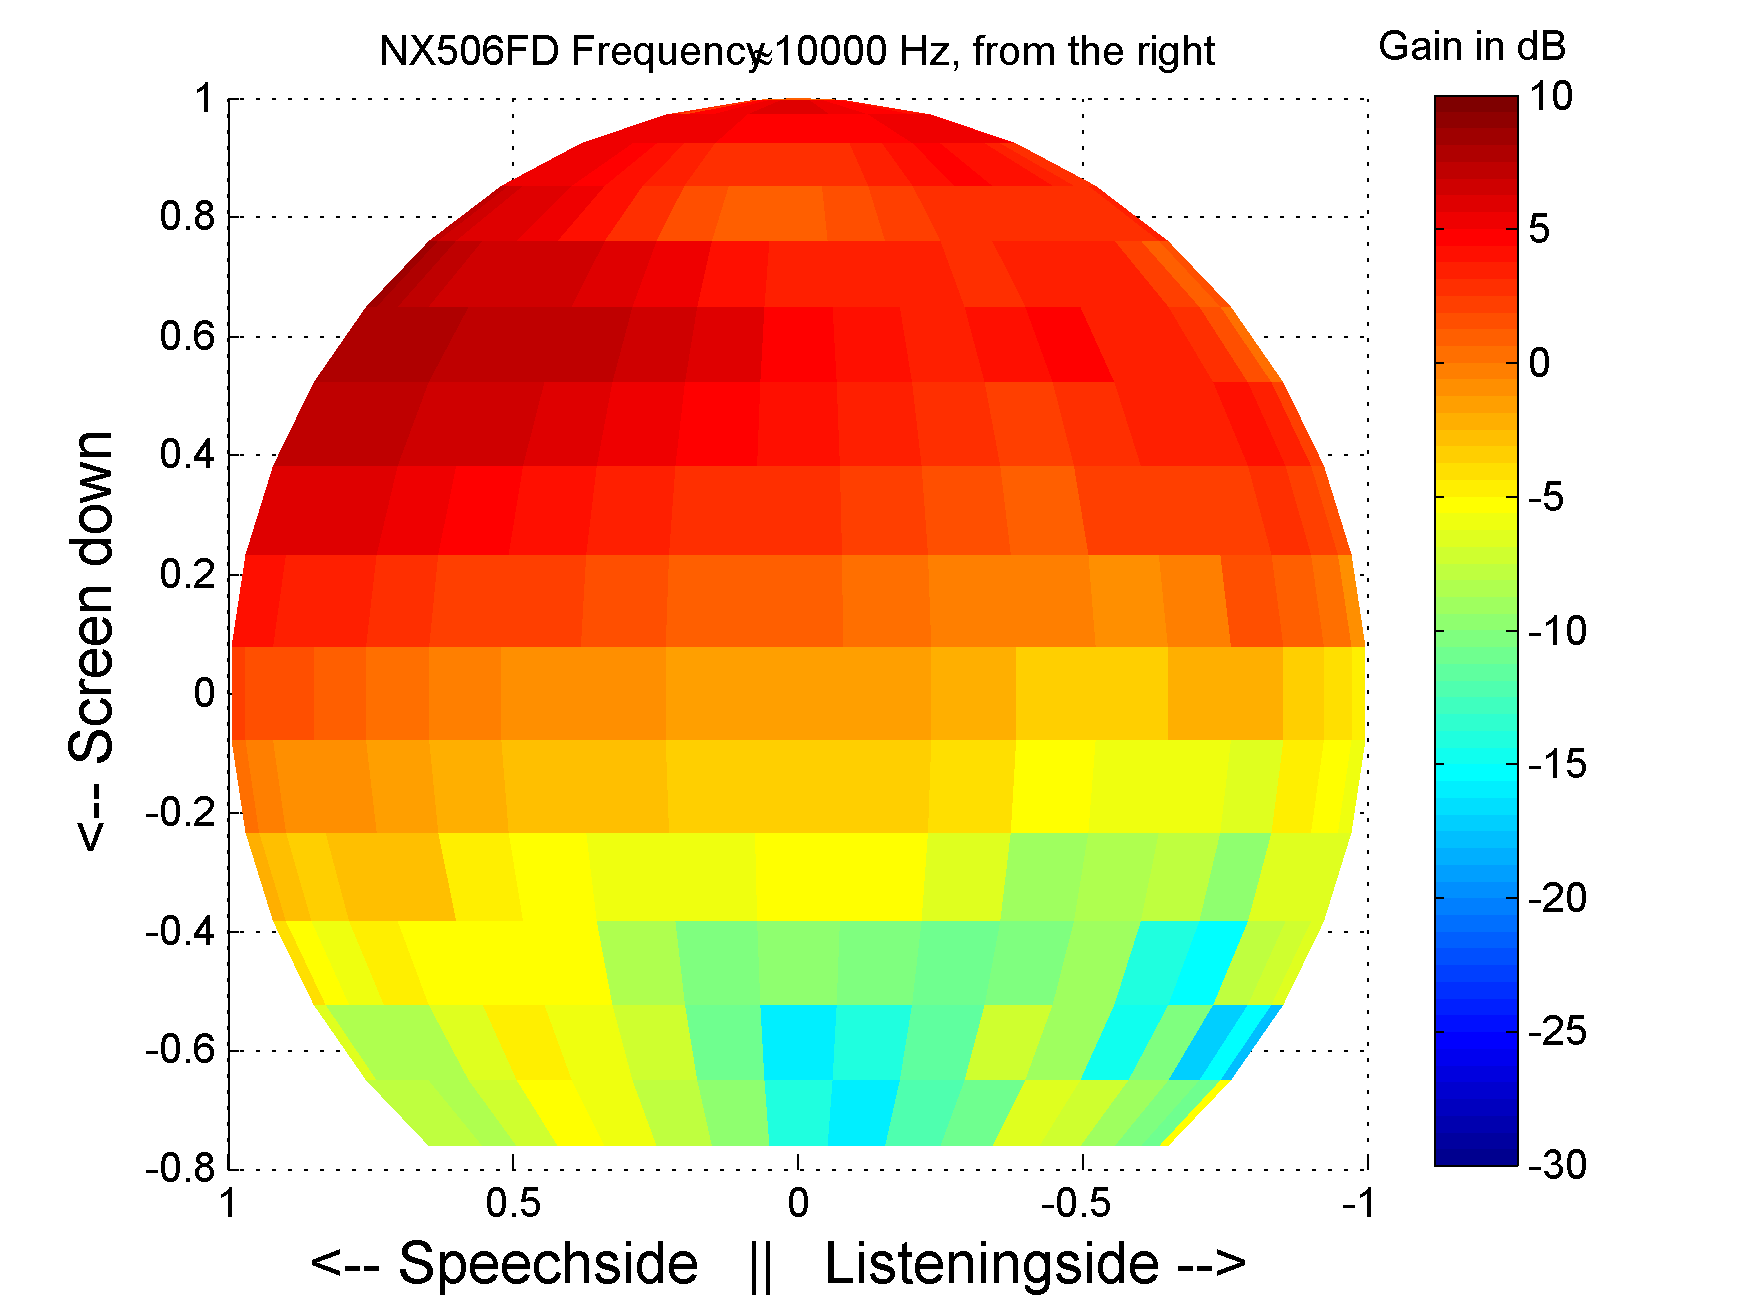
\includegraphics[height=0.28\textheight]{afbeeldingen/plots/results/NX506FD_10000_right.png}
        \end{subfigure}
\end{figure}

%%%%%%%%%%%%%%%%%%%%%%%%%%%%%%%%%%%%%%%%%%%%%%%%%%%%%%%%%%%%%%%%%%%%%%%%%%%%%%%%%%%%%%%%%%%%
% NX501 pluis
\clearpage
\begin{figure}[t!]
        \centering
        
        \caption[Measurement results {\nexus} (1), mid-air]{{\nexus}, labelled with number 1, measurements in mid-air, equalized}
        \label{fig:res_NX501_pluis}

        \begin{subfigure}[t]{0.5\textwidth}
			    \caption{$\phi=90^\circ$}
			    \label{fig:res_NX501_pluis_90}
                \centering
    			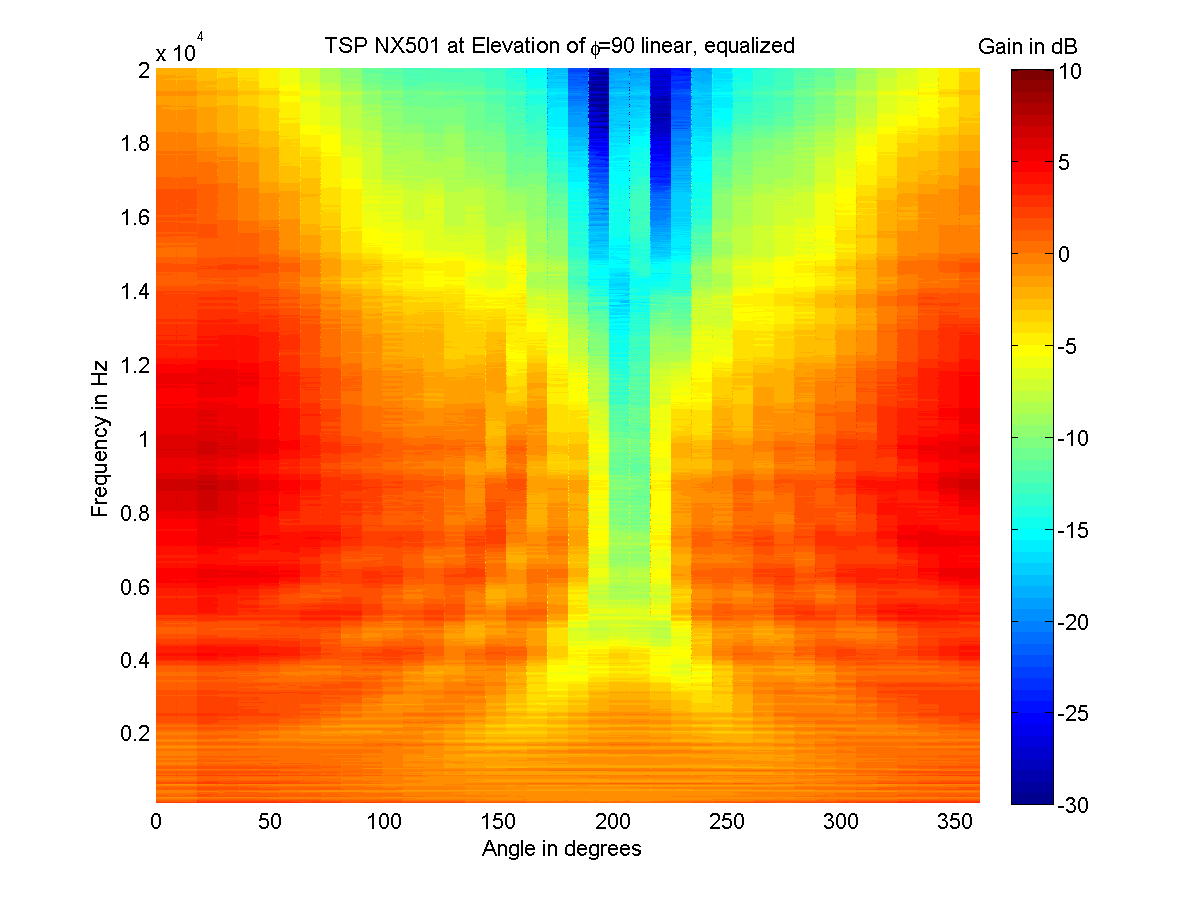
\includegraphics[height=0.28\textheight]{afbeeldingen/plots/results/NX501_TSP_090_lin_eq.png}
        \end{subfigure}~
        \begin{subfigure}[t]{0.5\textwidth}
			    \caption{$\phi=45^\circ$}
			    \label{fig:res_NX501_pluis_45}
                \centering
    			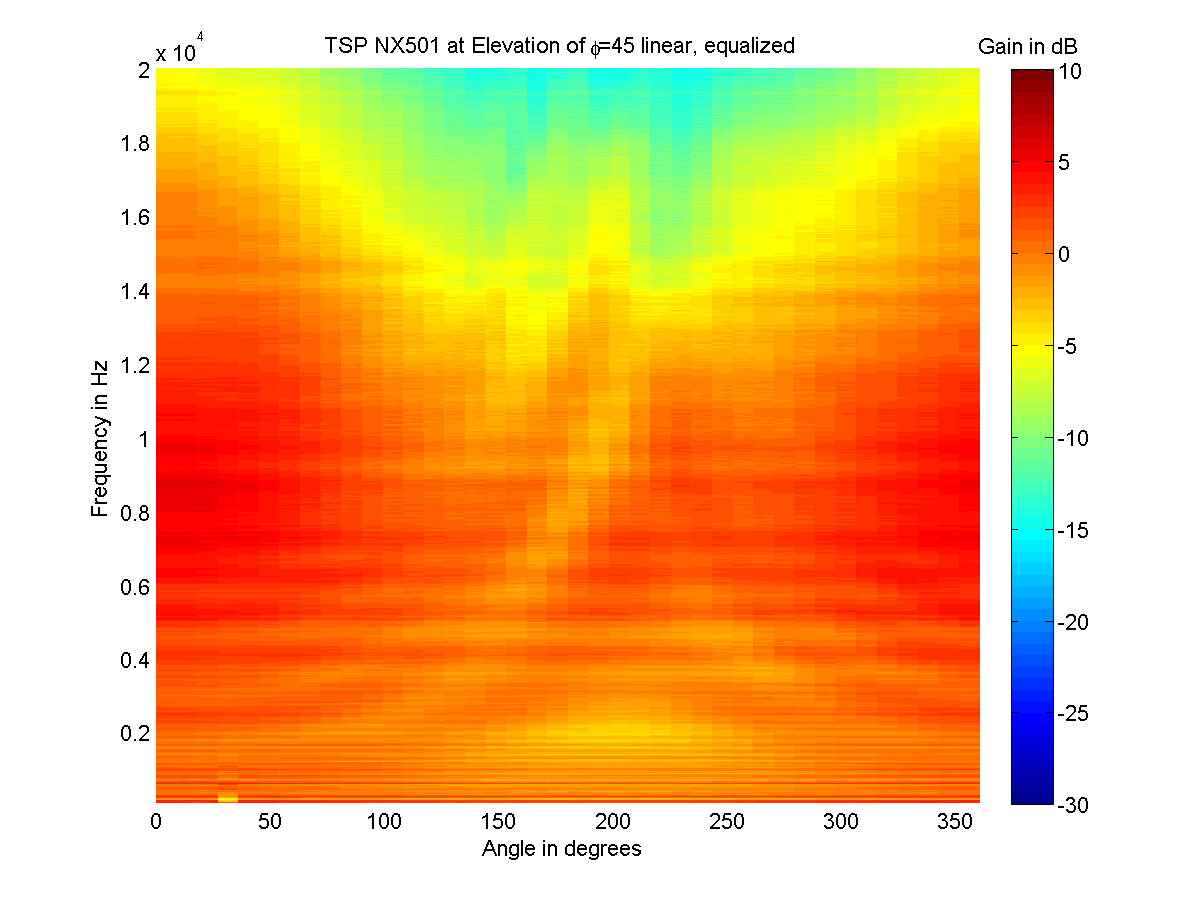
\includegraphics[height=0.28\textheight]{afbeeldingen/plots/results/NX501_TSP_045_lin_eq.png}
        \end{subfigure}
        
        \begin{subfigure}[t]{0.5\textwidth}
			    \caption{North pole: $\phi=0^\circ$}
			    \label{fig:res_NX501_pluis_0}
                \centering
    			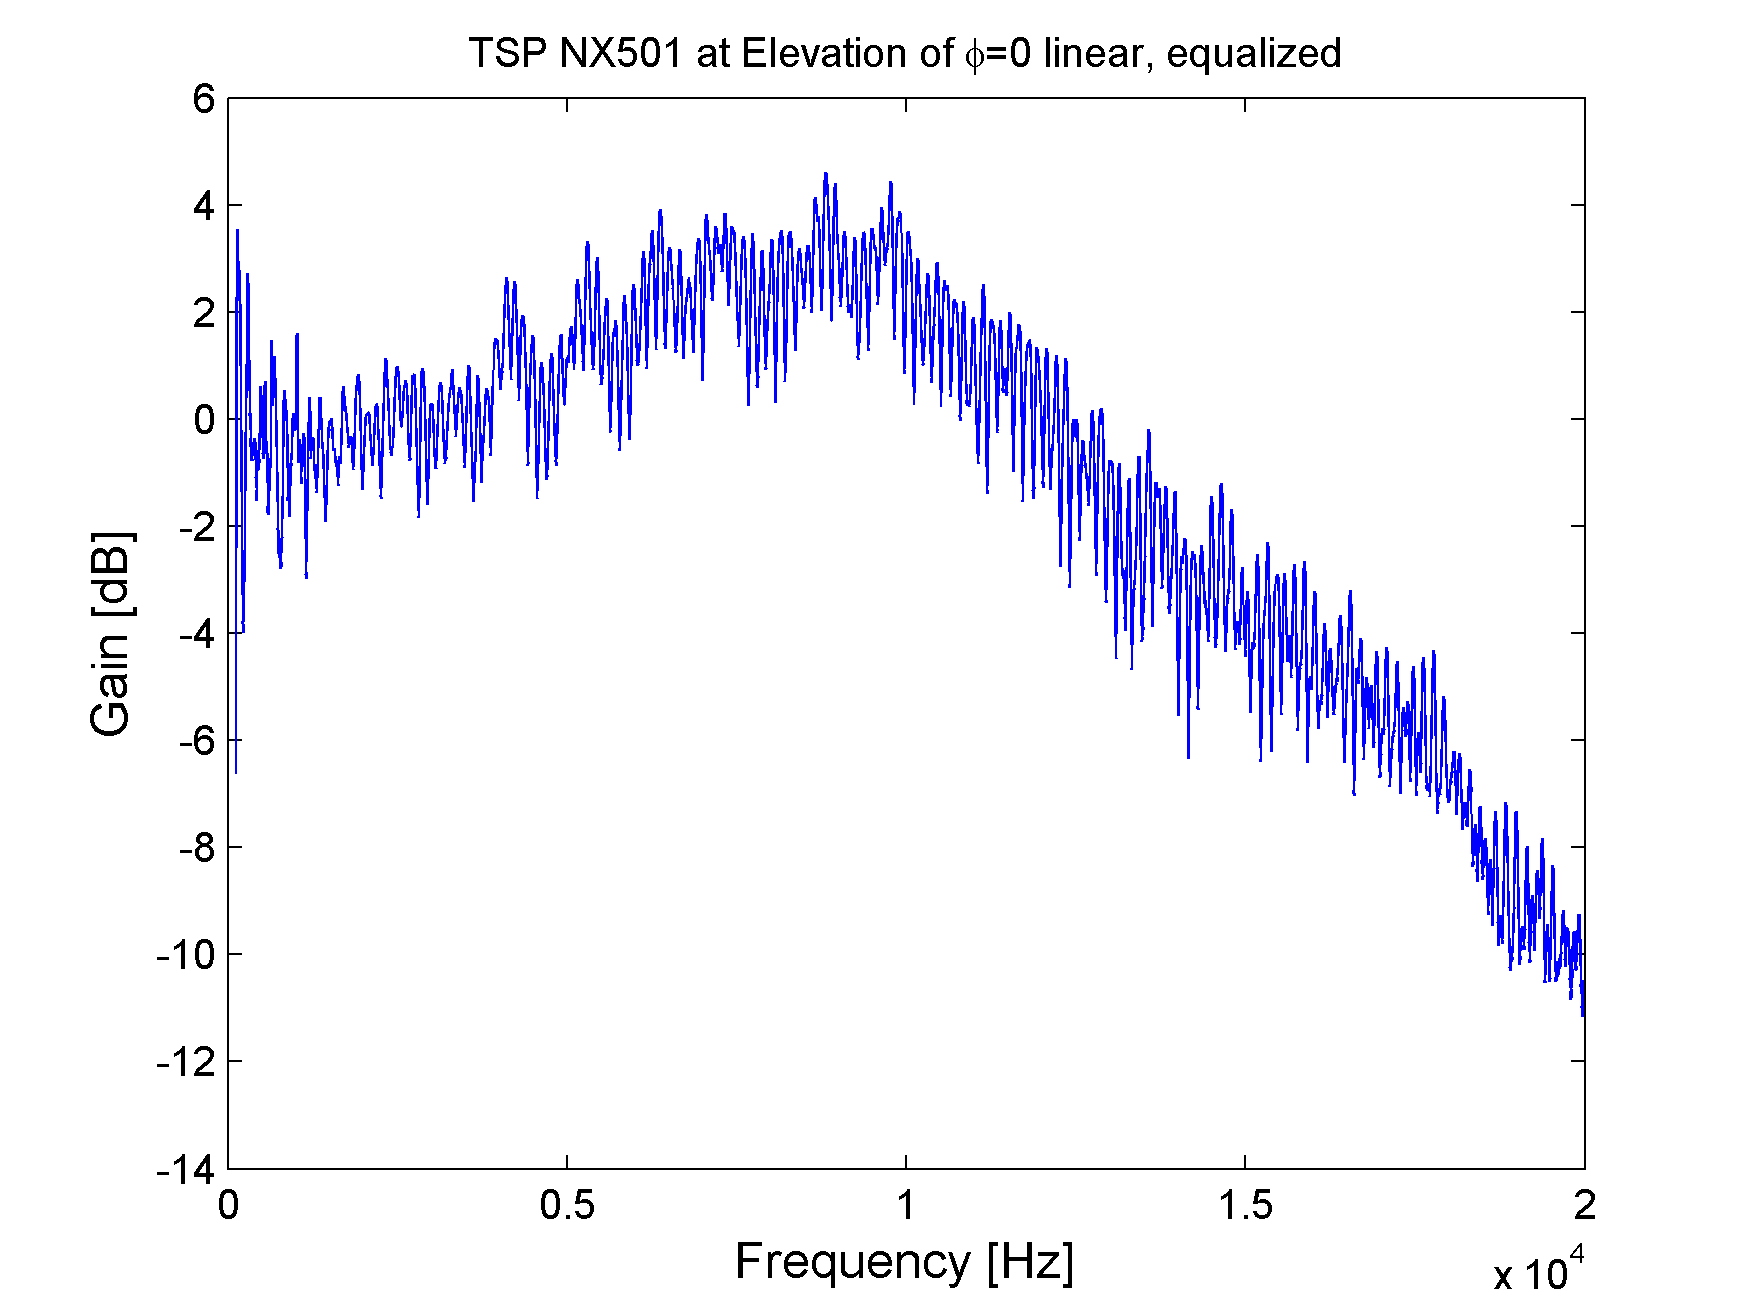
\includegraphics[height=0.28\textheight]{afbeeldingen/plots/results/NX501_north.png}
        \end{subfigure}
        
        \begin{subfigure}[t]{0.5\textwidth}
			    \caption{Upper half sphere $f=10000$ Hz, from the left}
			    \label{fig:res_NX501_pluis_sphere_left}
                \centering
    			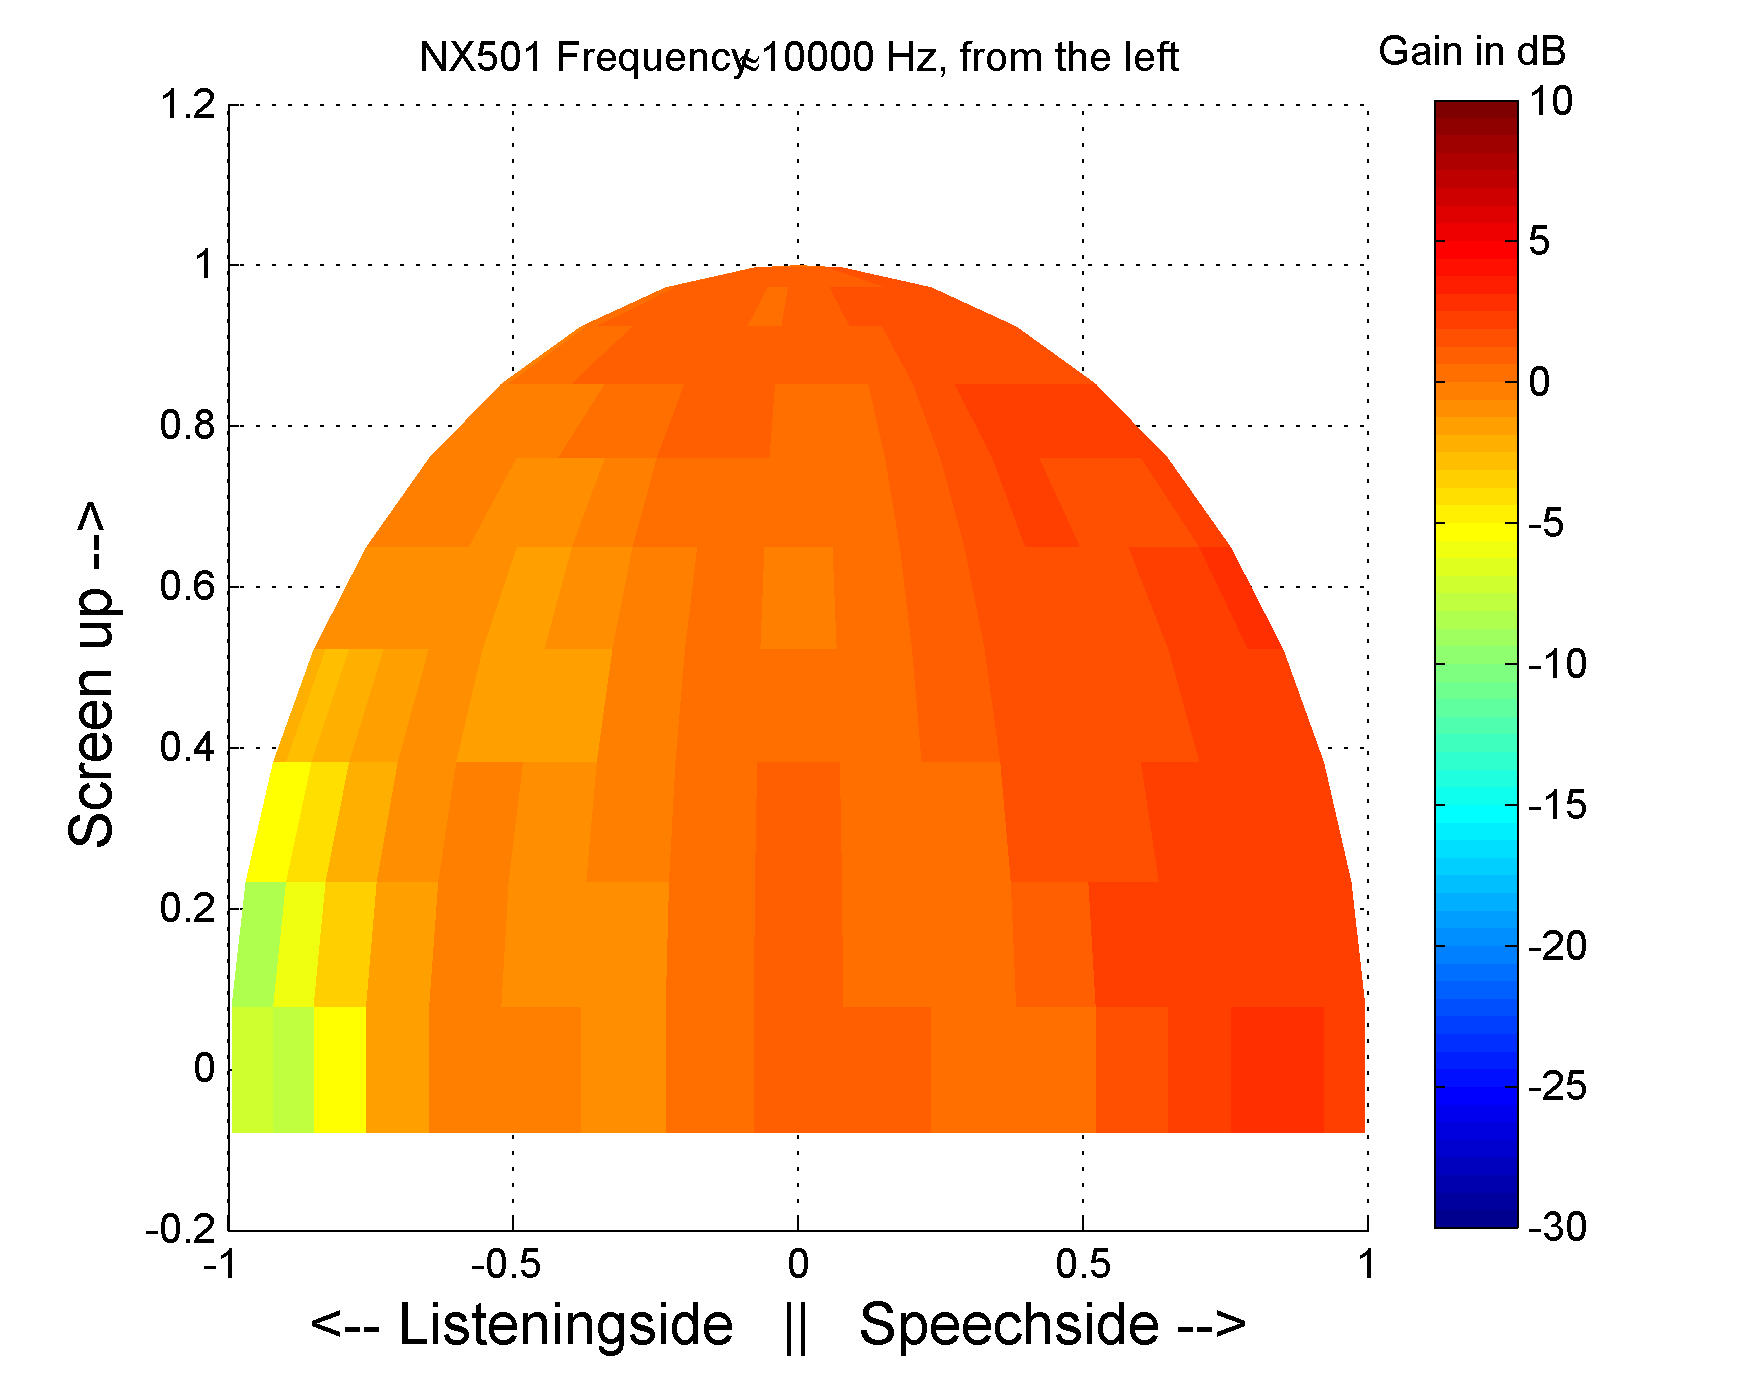
\includegraphics[height=0.28\textheight]{afbeeldingen/plots/results/NX501_10000_left.png}
        \end{subfigure}~
        \begin{subfigure}[t]{0.5\textwidth}
			    \caption{Upper half sphere $f=10000$ Hz, from the right}
			    \label{fig:res_NX501_pluis_sphere_right}
                \centering
    			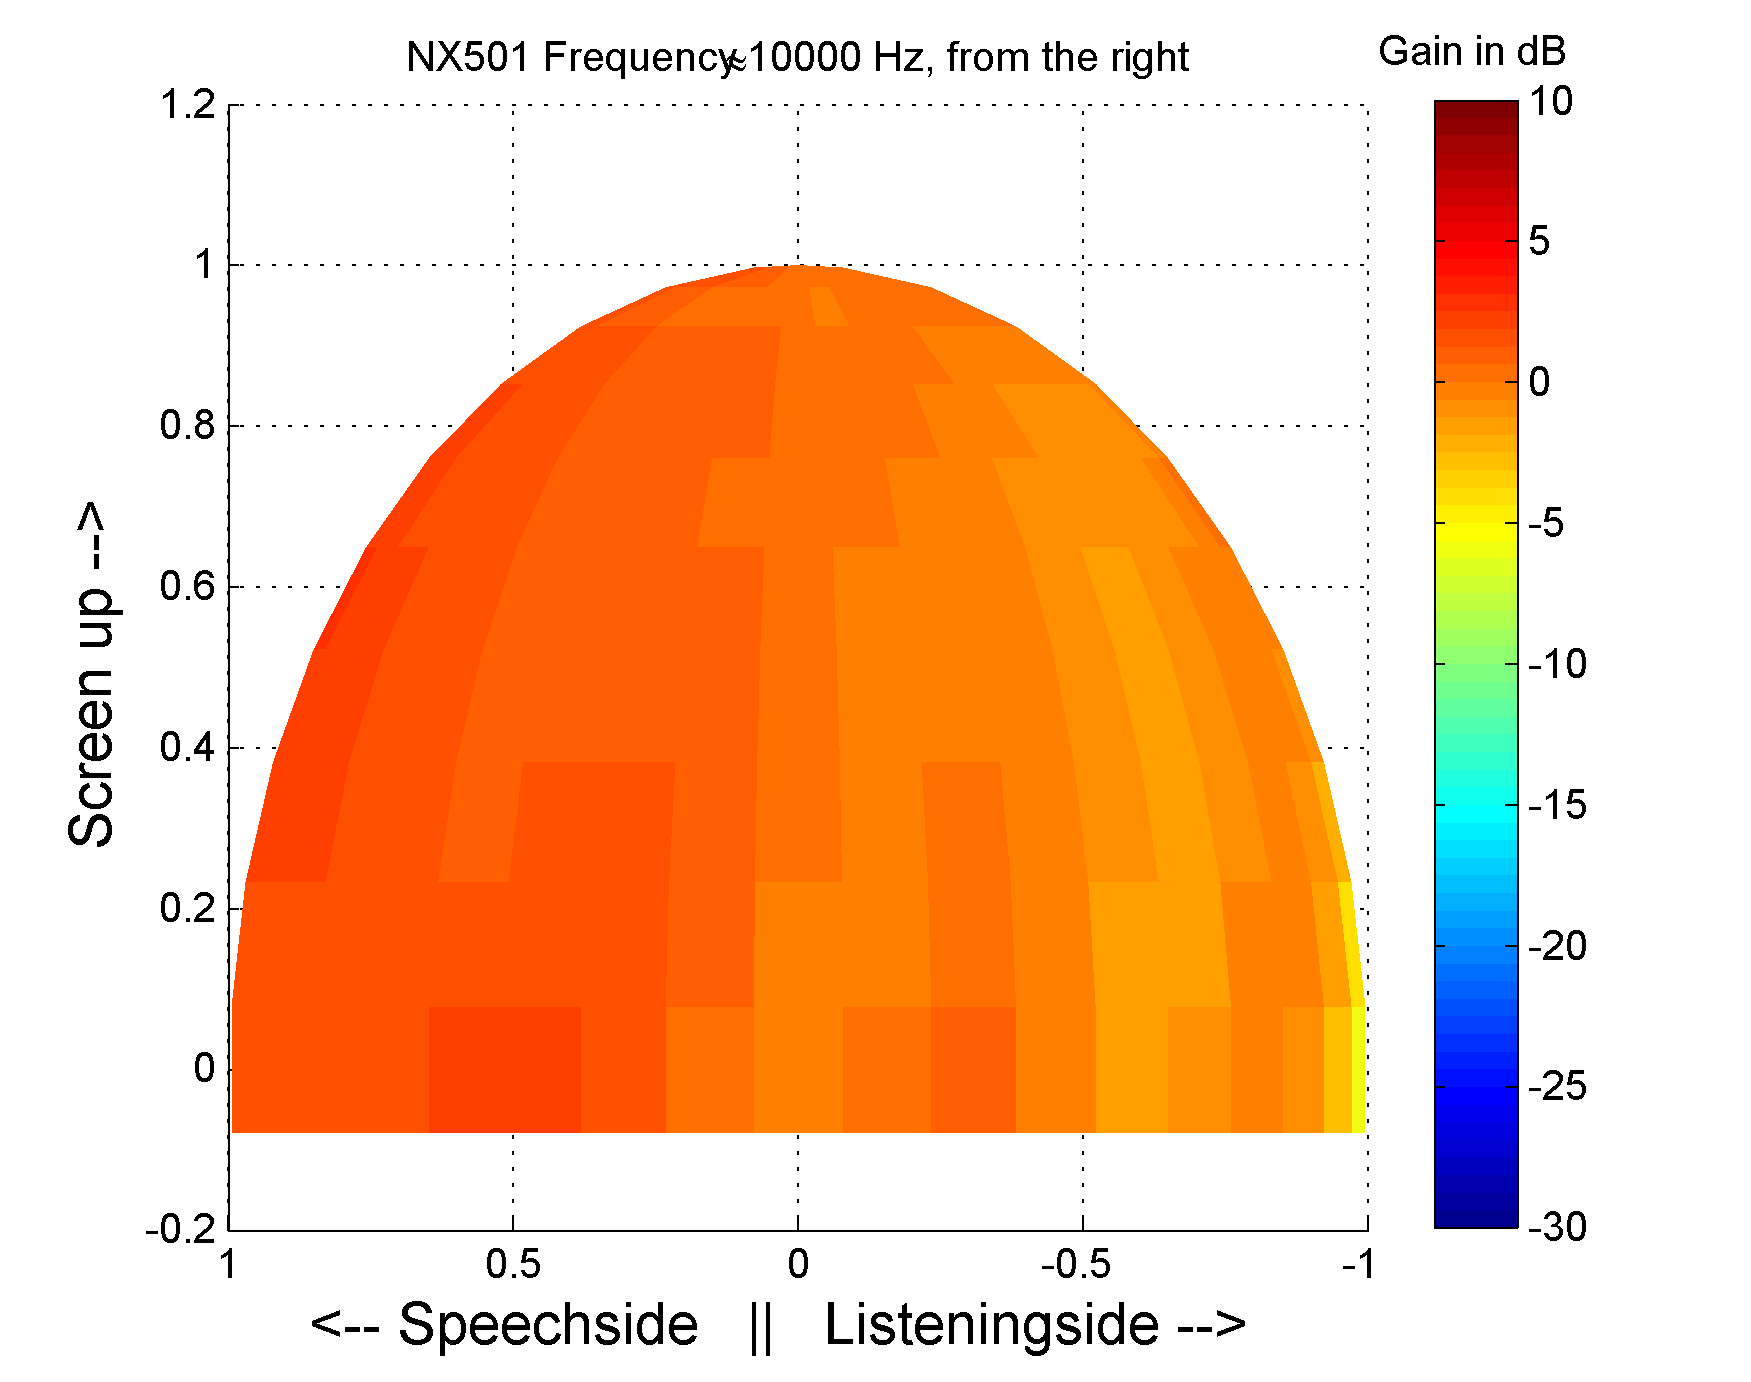
\includegraphics[height=0.28\textheight]{afbeeldingen/plots/results/NX501_10000_right.png}
        \end{subfigure}
\end{figure}